\documentclass[11pt,a4paper,twoside,pdf]{article}

% Paquetes (añade otros si los necesitas):

\usepackage[T1]{fontenc}
\usepackage[utf8]{inputenc}


\usepackage[pdftex,final]{graphicx}

% Style package
% Font Package (Palatino)
\usepackage{mathpazo}
% Packages for specific capabilities
\usepackage{rotating} % for text rotation in tables
\usepackage{multirow} % for multirow in tables
\usepackage{subfigure} % Place subfigures in figure environment
% Packages for specific symbols
\usepackage{amssymb}
\usepackage{amsmath}
\usepackage{amsfonts}
\usepackage{eurosym} % Euro symbol
\usepackage{bbding} % for \XSolidBrush
\usepackage{pifont} % for \ding{55} (a check mark)


\usepackage{latexsym}
\usepackage{soul}
\usepackage{array}
%\usepackage{marvosym}
\usepackage{epsfig}
\usepackage{graphics}
\usepackage{amsfonts}
\usepackage{xspace}
\usepackage{color}
\usepackage{booktabs}
\usepackage{xtab}
\usepackage[colorlinks=true,urlcolor=blue,linkcolor=blue,citecolor=blue]{hyperref}
\numberwithin{equation}{section}

\usepackage{lipsum}
\usepackage{pict2e}
\usepackage{wrapfig}
\usepackage{minted}

\linespread{1.05}

% TFG en inglés:
%\usepackage[english]{babel} 
%\addto\captionsenglish{\renewcommand{\chaptername}{}}

% TFG en español:
\usepackage[spanish,es-nodecimaldot,es-tabla,es-lcroman,es-nosectiondot,
            es-noindentfirst]{babel}
\renewcommand\spanishchaptername{}

% Formato de la página:
\usepackage{fancyhdr}
\usepackage[top=2.88cm,bottom=2.97cm,left=2.95cm,right=2.95cm]{geometry}
\setlength{\parskip}{0.1cm}

% Pon aquí tus definiciones:

\newcommand{\dis}{\displaystyle}
%\sodef\an{}{.2em}{1em plus1em}{2em plus.1em minus.1em}

\begin{document}

% Portada %%%%%%%%%%%%%%%%%%%%%%%%%%%%%%%%%%%%%%%%%%%%%%%%%%%%%%%%%%%%%%%%%%%%%%

\pagestyle{empty}


\noindent
\begin{tabular}{r}
\includegraphics[width=8.8cm]{img/escudoUGRmonocromo.png} \\[-1.8ex]
\hspace{31mm}\vspace{-8mm}
\begin{tabular}{c}
\hline\\[-1ex]\hskip-2mm
{\bf Facultad de Ciencias}\hspace{18mm}
\end{tabular}
\end{tabular}

\large
\vspace{30mm}
\hspace{25mm}
\begin{tabular}{l}
GRADO EN F\'ISICA
\end{tabular}

\vspace{45mm}
\hspace{25mm}
\begin{tabular}{l}
TRABAJO FIN DE GRADO
\\[1.5ex]
\vspace{0.1cm}
\LARGE\bf Diseño y evaluación de una antena\\
\vspace{0.1cm}
\LARGE\bf fabricada mediante impresión 3D\\
\LARGE\bf y galvanización
\end{tabular}
%
\vfill
\hspace{25mm}
\begin{tabular}{l}
Presentado por:
\\
{\bf D. Alejandro José Zarzuela Moreno}
\\[3ex]
Curso Académico 2024/2025
\end{tabular}
%

%%%%%%%%%%%%%%%%%%%%%%%%%%%%%%%%%%%%%%%%%%%%%%%%%%%%%%%%%%%%%%%%%%%%%%%%%%%%%%%%
%%%%%%%%%%%%%%%%%%%%%%%%%%%%%%%%%%%%%%%%%%%%%%%%%%%%%%%%%%%%%%%%%%%%%%%%%%%%%%%%

\newpage
%
\begin{center}
{\bf Resumen}
\bigskip

\begin{minipage}{0.8\linewidth}
En este trabajo se ha explorado el diseño, fabricación y evaluación de una antena TEM de bocina mediante técnicas de impresión 3D, electroplating, simulación y medidas experimentales. El diseño ha consistido en un proceso iterativo de diseño, impresión 3D y electroplating en el que se han corregido paso a paso los problemas que presentaba la antena. Para ello se ha partido de las medidas que presenta Mallahzadeh en su artículo \cite{tem_horn} y se han introducido las modificaciones necesarias para adaptarla a este método de construcción mediante el procedimiento anterior. Se han explicado en detalle los pasos para su construcción y electroplating dado que uno de los objetivos de este trabajo es explorar las posibilidades de un método de creación de antenas fácilmente reproducible. Posteriormente se ha analizado el parámetro $S_{11}$ de la antena real mediante un analizador vectorial de redes y se ha comparado con el resultado de una simulación de la misma, comentando la similitud entre ellos y comparándolos también con los del artículo anterior.
\end{minipage}

\vfill

{\bf Abstract} 
\bigskip

\begin{minipage}{0.8\linewidth}
This project has explored the design, fabrication and evaluation of a TEM horn antenna using 3D printing, electroplating, simulation and experimental measurements techniques. The design consisted  of an iterative process of design, 3D printing and electroplating in which the issues presented by the antenna were corrected step by step. The measurements presented by Mallahzadeh in his article \cite{tem_horn} were used as a starting point and the necessary adjustments were made to adapt it to this construction method using the aforementioned procedure. The steps for its construction and electroplating were explained in detail since one of the objectives of this project is to explore the possibilities of an easily reproducible antenna creation method. Subsequently, the $S_{11}$ parameter of the real antenna was analyzed using a vector network analyzer and compared with the results of a simulation of the same, commenting on the similarity between them and also comparing them with those of the previous article.
\end{minipage}
\newpage
{\bf Agradecimientos}
\bigskip

\begin{minipage}{\linewidth}
Este TFG ha sido posible gracias a la colaboración de muchas personas. En primer lugar, quiero agradecer enormemente a mis tutores Luis Manuel Díaz Angulo y Miguel Ángel Fernández Rodríguez por su interés en el proyecto, su ayuda en todos los ámbitos y su trato tan cercano. También le doy las gracias a mi mentor Antonio Rubio Andrés por su apoyo y colaboración en tantas sesiones de laboratorio. Además, agradezco al personal de Bibliomaker de la Facultad de Ciencias por darme acceso y asistirme en el uso de sus impresoras; a Federico Coca Caba, presidente del Club Robótica Granada, por crear una antena usando su impresora; al equipo de Elemwave por darme acceso a su software de simulación y a Adrián Arce por su gran ayuda en la instalación y acceso al mismo; a Mario Fernández Pantoja por su colaboración para realizar las medidas experimentales de $S_{11}$ mediante VNA; y a Juan Luis Godino Rodríguez por algunas de las fotos que se verán en este texto.
\end{minipage}

\vfill

\end{center}

%%%%%%%%%%%%%%%%%%%%%%%%%%%%%%%%%%%%%%%%%%%%%%%%%%%%%%%%%%%%%%%%%%%%%%%%%%%%%%%%
%%%%%%%%%%%%%%%%%%%%%%%%%%%%%%%%%%%%%%%%%%%%%%%%%%%%%%%%%%%%%%%%%%%%%%%%%%%%%%%%
%\newpage

\tableofcontents


%%%%%%%%%%%%%%%%%%%%%%%%%%%%%%%%%%%%%%%%%%%%%%%%%%%%%%%%%%%%%%%%%%%%%%%%%%%%%%%%
%%%%%%%%%%%%%%%%%%%%%%%%%%%%%%%%%%%%%%%%%%%%%%%%%%%%%%%%%%%%%%%%%%%%%%%%%%%%%%%%
\newpage

\pagestyle{fancy}
\fancyhead[RO,LE]{\leftmark}
\fancyhead[LO,RE]{\thepage}
\fancyfoot{}

\normalsize

\section{Introducción}

Las antenas son partes fundamentales de los circuitos de radiofrecuencia y las telecomunicaciones. Si bien las técnicas de construcción tradicionales o industriales dan resultados consistentes y muy precisos en general, el prototipado tiene poca cabida en ellas y ciertas partes de su proceso requieren maquinaria especializada. Es por esto que el objetivo de este TFG es explorar la construcción de antenas mediante impresión 3D y electrodepositado, que son mucho más accesibles. \\

Mediante impresión 3D tendremos acceso a formas y figuras que serían muy complicadas de crear de otra forma. Esto nos dará gran libertad en cuanto a diseño, por lo que se realizará multitud de pasos de prototipado que permitirán personalizar la antena según nuestras necesidades. 

Tras la construcción de la antena será necesario hacerla conductora, por lo que se usará el método de la electrodeposición o electroplating para depositar una fina capa conductora sobre ella. Debido al grosor de la capa que se creará y a las frecuencias que la antena tendrá como objetivo, el efecto skin (que se discutirá más adelante) hará que no sea un problema el hecho de que la antena no esté hecha de metal macizo. \\

Una herramienta que va de la mano con el objetivo de este proyecto es la simulación. Esta nos permite predecir el comportamiento aproximado que tendrá una antena tras los distintos cambios que se llevan a cabo en el prototipado, dándonos la capacidad de elegir la forma en la que se quieren implementar las modificaciones para tener un mejor resultado, ahorrándonos los pasos de impresión y metalizado y sus respectivos materiales en varias ocasiones.

Para el análisis de los resultados de la simulación serán importantes conceptos como impedancia característica, longitud eléctrica, ondas incidentes y reflejadas, coeficiente de reflexión o impedance matching, que se discutirán a lo largo del texto.

Mediante esos mismos conceptos se pueden analizar las propiedades de las antenas reales que se construirán usando el instrumental adecuado para medirlas, lo que también permite hacer comparaciones con la simulación para intentar entender qué partes del proceso de fabricación afectan al rendimiento de esas antenas y tener así una guía que nos devuelve al paso de diseño 3D.\\


%%%%%%%%%%%%%%%%%%%%%%%%%%%%%%%%%%%%%%%%%%%%%%%%%%%%%%%%%%%%%%%%%%%%%%%%%%%%%%%%
%%%%%%%%%%%%%%%%%%%%%%%%%%%%%%%%%%%%%%%%%%%%%%%%%%%%%%%%%%%%%%%%%%%%%%%%%%%%%%%%
\section{Fundamento teórico}

%% Línea argumental: 
% Contexto -> Líneas de transmisión/impedancia característica -> Fenómenos de reflexión -> VSWR/impedance matching -> Tapering -> Fundamentos de antenas -> Partes de la TEM horn -> ? -> Justificar el uso de este tipo de antena (ancho de banda, direccionalidad, ...)

Los sistemas eléctricos que son de interés para este TFG consisten en un generador que proporciona energía (y, con ella, información), un sistema que la recibe (una antena con sus diferentes partes) y una línea de transmisión que los conecta, como se aprecia en la figura \ref{fig:esqmLineaTransmision} (izq). Debido a los fenómenos que se discutirán a continuación, en general será necesario estudiar la línea de transmisión usando un marco teórico distinto al de la teoría de circuitos (TC).\\

Cuando la longitud de onda con la que trabaja un circuito eléctrico es mucho mayor que las dimensiones del mismo se pueden aplicar aproximaciones que simplifican su análisis, esto es, la teoría de circuitos. Esto no pasa en el caso de las líneas de transmisión, donde los parámetros como fase y magnitud de las corrientes y voltajes varían a lo largo de su extensión. Dado que las líneas de transmisión están siempre formadas por al menos dos conductores, se suelen representar mediante dos cables y se analizan mediante el modelo de parámetros distribuidos, en el que se estudia mediante TC el equivalente a un segmento de línea de transmisión de longitud $\Delta z$ como el de \ref{fig:esqmLineaTransmision} (der).

\begin{figure}[!h] \label{fig:esqmLineaTransmision}
\begin{minipage}[c]{.49\linewidth}
\includegraphics[width=0.9\linewidth]{img/fundTeo/LTAlfonso.png}
\end{minipage}\hfill
\begin{minipage}[c]{.49\linewidth}
\includegraphics[width=\linewidth]{img/fundTeo/lineaTransmision.png}
\end{minipage}
\caption{A la izquierda: esquema de un sistema eléctrico con línea de transmisión \cite{alfonsoSalinas}; a la derecha: circuito equivalente a un segmento de línea de transmisión de longitud $\Delta z$ \cite{pozar}.}
\label{fig:esqmLineaTransmision}
\end{figure}

La resistencia $R$, inductancia $L$, conductancia $G$ y capacidad $C$ son propiedades características de la línea de transmisión y son causadas por la distribución espacial de los conductores y del medio que los separa, así como por sus propiedades físicas. 

Cuando en el circuito de la figura \ref{fig:esqmLineaTransmision} (der) se aplican las leyes de Kirchhoff, luego se divide por $\Delta z$ y finalmente se toma el límite cuando $\Delta z\rightarrow0$ se obtienen las llamadas ecuaciones del Telégrafo \cite{pozar} que, tras describir mediante fasores y resolver, dan como solución
\begin{equation}\label{eq:solViajeras}
    \begin{split}
        V(z) &= V_0^+e^{-\gamma z} + V_0^-e^{\gamma z} \\
        I(z) &= I_0^+e^{-\gamma z} + I_0^-e^{\gamma z}
    \end{split}
\end{equation}
\noindent donde los términos $e^{-\gamma z}$ corresponden a ondas propagándose en dirección $+z$ y viceversa. Por la distribución del sistema con el que trabajamos, a las ondas que viajan en dirección $+z$ las llamaremos \textit{ondas incidentes}, y a las que viajan en sentido contrario \textit{ondas reflejadas}.\\

Operando con estos fasores se obtiene la expresión de la llamada impedancia característica de la línea
\begin{equation}
    Z_0 = \frac{R+j\omega L}{\gamma} = \sqrt{\frac{R+j\omega L}{G+j\omega C}}
\end{equation}

Como $Z_0$ viene dada por $R$, $L$, $G$ y $C$, es característica de la línea de transmisión y su valor depende de las propiedades físicas y distribución en el espacio de los elementos que conforman la línea. En nuestro caso tratamos con una línea de transmisión coaxial, cuya impedancia característica es
\begin{equation}\label{impedCaractCoax}
    Z_0 = \sqrt{\frac{\mu}{\epsilon}} \frac{\ln b/a}{2\pi},
\end{equation}
\noindent donde $a$ es el radio del conductor interno, $b$ el del externo y $\mu$ y $\epsilon$ son la permeabilidad magnética y permisividad eléctrica del dieléctrico que los separa \cite{pozar}. La línea de transmisión con la que trabajaremos tiene una impedancia característica de 50 $\Omega$.\\

$Z_0$ es un parámetro muy importante en el estudio de las líneas de transmisión porque su valor determina el tipo de carga que puede gestionar el sistema debido a las reflexiones que aparecen en él. Este fenómeno se ilustra a continuación con un ejemplo:

Sea una línea de transmisión sin pérdidas ($R=G=0$) con impedancia característica $Z_0$. Si desde la fuente se emite una onda incidente $V_0^+e^{-j\beta z}$, la relación entre ese voltaje y la corriente vendrá dada por $Z_0$. Si en los extremos de la línea se aplica una impedancia de carga $Z_L\neq Z_0$, la relación entre el voltaje y la corriente variará necesariamente, por lo que aparecerá una onda reflejada para que esto ocurra. El voltaje y la corriente de la línea de transmisión serán ahora
\begin{equation*}
\begin{split}
    V(z) &= V_0^+e^{-j\beta z} + V_0^-e^{j\beta z}\\[3pt]
    I(z) &= \frac{V_0^+}{Z_0}e^{-j\beta z} + \frac{V_0^-}{Z_0}e^{j\beta z}
\end{split}
\end{equation*}

En $z=0$ se debe cumplir 
\begin{equation}
    Z_L = \frac{V(0)}{I(0)} = \frac{V_0^++V_0^-}{V_0^+-V_0^-}Z_0 \hspace{0.5cm}\Rightarrow\hspace{0.5cm} V_0^- = \frac{Z_L-Z_0}{Z_L+Z_0}V_0^+
\end{equation}

De este modo se puede definir el coeficiente de reflexión de voltaje
\begin{equation}
    \Gamma = \frac{V_0^-}{V_0^+} = \frac{Z_L-Z_0}{Z_L+Z_0},
\end{equation}
\noindent por lo que las ondas de voltaje y corriente a lo largo de la línea se pueden escribir como
\begin{equation}\label{eq:Gamma}
\begin{split}
    V(z) &= V_0^+(e^{-j\beta z} + \Gamma e^{j\beta z})\\
    I(z) &= \frac{V_0^+}{Z_0}(e^{-j\beta z} + \Gamma e^{j\beta z})
\end{split}
\end{equation}

Conociendo el valor del coeficiente de reflexión $\Gamma$ se puede calcular la relación entre el voltaje máximo y el mínimo de la onda estacionaria. Esta relación es un número real que recibe el nombre de $VSWR$ (Voltage Standing Wave Ratio), y se calcula como
\begin{equation}\label{eq:VSWR}
    VSWR = \frac{V_{max}}{V_{min}} = \frac{1+|\Gamma|}{1-|\Gamma|}.
\end{equation}

Desde el punto de vista del sistema, para que la transferencia de potencia desde la fuente a la carga sea máxima se debe cumplir la condición de \textit{impedance matching}, es decir, la impedancia de la carga debe ser la misma que la impedancia característica de la red de transmisión o, lo que es lo mismo, $VSWR = 1$. Esto en general es importante porque valores altos de $VSWR$ pueden dar lugar a un comportamiento no deseado en la carga o incluso a daños en el generador.\\

Otra forma de estudiar esto es mediante el parámetro de scattering $S_{11}$, que está directamente relacionado con el $VSWR$. En un sistema con varios puertos se define $S_{ij}$ como el coeficiente de transmisión si se envía una onda incidente de voltaje $V_j^+$ por el puerto $j$ y se mide el voltaje de la onda reflejada $V_i^-$ en el puerto $i$ cuando el resto de puertos cumplen impedance matching \cite{pozar}. Para una antena como la nuestra, que solo tiene un puerto, el parámetro $S_{11}$ expresado en dB será
\begin{equation}\label{eq:S11}
    |S_{11}|_{dB} = 20\log \left(\frac{Z_L-Z_0}{Z_L+Z_0}\right)
\end{equation}

Como ya se ha dicho, el objetivo es conectar a la línea de transmisión una antena TEM de bocina que radiará directamente al aire. Dado que la línea de transmisión que usaremos tiene una impedancia característica $Z_0=50$ $\Omega$ y el aire tiene una impedancia de 377 $\Omega$, en el diseño de la antena se ha empleado un \textit{tapering} exponencial, en concreto, el que que se desarrolla en la ecuación \ref{eq:w} de la sección \ref{sec:dis}.

El tapering es una técnica que consiste en variar las dimensiones y forma de la antena a lo largo de su extensión para modificar el valor de la impedancia característica gradualmente y minimizar así el efecto de las reflexiones.\\

A continuación se discutirá en mayor profundidad el funcionamiento de una antena. En general, una antena es un dispositivo que se encarga de emitir o recibir ondas electromagnéticas, por lo que se puede ver como el elemento que actúa como transición entre el circuito y el espacio libre por el que viajan dichas ondas.\\

Las dos propiedades más importantes que debe tener una antena son, por un lado, la máxima transferencia de potencia entre el circuito y el espacio libre y, por otro lado, la forma de su patrón de emisión o recepción.

Para maximizar la transferencia de potencia se deben aplicar un impedance matching y tapering adecuados, y para que su direccionalidad sea la deseada debe tomar una forma específica. Esto da lugar a muchos tipos diferentes de antena como las de dipolo, las parabólicas o las TEM de bocina, como la que usaremos.
\begin{figure}[!h]
    \centering
    \includegraphics[width=0.64\linewidth]{img/fundTeo/dipolo1.png}
    \vspace{-0.3cm}
    \caption{Esquema de las líneas de campo eléctrico emitidas por una antena formada por dos cables conductores \cite{balanis}.}
    \label{fig:dipolo1}
\end{figure}

En general, una antena TEM funcionará de manera similar a la de la figura \ref{fig:dipolo1}, donde aparece un esquema de una antena formada por dos cables o alambres conectada mediante una línea de transmisión a una fuente de corriente alterna. Cuando la fuente genera una diferencia de potencial en la línea, aparece un campo eléctrico que va de un cable hasta el otro transversalmente. Como las cargas se están moviendo, aparecerá un campo magnético que será perpendicular tanto a los cables como al campo $\mathbf{E}$. Conforme la fuente invierte la tensión aplicada, los campos entre los cables cambian de sentido e intensidad.

En el otro extremo de la línea de transmisión se encuentra la antena, que en este ejemplo no es más que una continuación de la línea con los extremos abiertos y alejándose entre sí. Esto da lugar a que las líneas de campo que viajaban a lo largo de la línea acaben liberándose de los cables conductores y se sigan propagando por el espacio vacío, ahora en forma de ondas libres cerradas formándose al ''unir'' los extremos de los diferentes frentes, tal como se aprecia en la figura \ref{fig:dipolo1} para el campo eléctrico. En este ejemplo los pulsos se pueden delimitar también observando que los puntos $P_0$ y $P_2$ están en fase.
\begin{wrapfigure}{r}{6.2cm}
    \vspace{-0.12cm}
    \includegraphics[width=\linewidth]{img/fundTeo/antenaMallahzadeh.png}
    \vspace{-0.7cm}
    \caption{Esquema de la antena TEM de bocina que se construirá \cite{tem_horn}.}
    \label{fig:antenaMallahzadeh}
\end{wrapfigure}

En la práctica, y para una antena con geometría compleja como la que se usará, las ondas no solo se emitirán, sino que una parte de los campos rebotará al alcanzar los bordes de la antena, lo que dará lugar a pérdidas y cambios en el patrón de emisión.

En el caso de nuestra antena, como la línea de transmisión es coaxial el diseño no será tan simple como conectar cada placa con su terminal correspondiente de la línea. Es necesario crear una estructura que conecte la línea de transmisión a la antena y que introduzca la mínima cantidad de distorsión a la señal. Esta estructura, la alimentación o \textit{feed} de la antena, consistirá en dos bloques paralelos separados una cierta distancia $d_0$. Desde cada bloque saldrá una placa de la antena, como se observa en la figura \ref{fig:antenaMallahzadeh}. El bloque inferior tendrá un hueco por el que pasará el cable coaxial, de manera que el conductor central del cable (o ''vivo'') hace contacto con el bloque superior del feed, y el conductor exterior (o ''tierra'') hace contacto con el bloque inferior. Otros elementos como la placa de corto o el soporte del feed y sus dimensiones son también relevantes, pero dado que nuestro objetivo no es el diseño desde cero de la antena no se discutirán en profundidad y se usarán las medidas que ofrece Mallahzadeh \cite{tem_horn}.\\

Uno de los motivos por los que se ha elegido este modelo de antena es su gran ancho de banda $B$. El ancho de banda es la anchura del intervalo de frecuencias en el que el $|S_{11}|$ de la antena es menor que un cierto valor de referencia, típicamente -10 dB. Para este modelo de antena, dicho intervalo de frecuencias va desde los 2 GHz hasta los 14.2 GHz con $|S_{11}|\leq-10$ dB \cite{tem_horn}. 

Esta propiedad le da gran versatilidad a la antena porque permite que se opere en diferentes bandas de frecuencias, y para anchos de banda tan amplios incluso se puede usar en radares ya que la duración mínima $\tau$ de los pulsos emitidos es inversamente proporcional al ancho de banda $B$, de manera que la resolución de la antena permitirá distinguir objetos a distancias a partir de 
\begin{equation}
    \Delta R = \frac{c\tau}{2}\propto\frac{c}{2B}
\end{equation}
por lo que se podrán distinguir objetos muy cercanos para anchos de banda altos \cite{radar} o, dicho de otro modo, tendrá alta resolución.\\

Un fenómeno que aparece para las frecuencias en las que trabajaremos es el efecto skin \cite{pozar}. Mientras que en corriente continua la densidad de corriente se distribuye de forma prácticamente homogénea, en corriente alterna se acumula en la superficie del conductor. Esto sucede porque la corriente alterna da lugar a campos magnéticos variables en el tiempo que, por la ley de Faraday, inducen corrientes parásitas en el interior del conductor que se oponen al flujo de corriente primario. Como este efecto es mayor en el centro de la sección del conductor, las corrientes primarias tienden a viajar por la superficie.

Para cuantificar su efecto y evaluarlo en función de la frecuencia se define la profundidad de penetración
\begin{equation}
    \delta = \sqrt{\frac{2}{\omega\mu\sigma}} = \sqrt{\frac{1}{\pi f\mu\sigma}},
\end{equation}
que no es más que la profundidad en el conductor a la que la magnitud de los campos se habrá disminuido en un 36.8\%. Como se usará un recubrimiento de cobre ($\mu\simeq\mu_0$ y $\sigma=5.8\cdot10^{7}$ S/m), se obtiene los valores $\delta(f=2\text{ GHz})=1.478$ $\mu$m y $\delta(f=6\text{ GHz})=0.853$ $\mu$m. Como veremos en secciones posteriores, el objetivo es aplicar un recubrimiento de unas 17 micras, por lo que supuestamente será suficiente para no interrumpir la propagación de las corrientes.


%%%%%%%%%%%%%%%%%%%%%%%%%%%%%%%%%%%%%%%%%%%%%%%%%%%%%%%%%%%%%%%%%%%%%%%%%%%%%%%%
%%%%%%%%%%%%%%%%%%%%%%%%%%%%%%%%%%%%%%%%%%%%%%%%%%%%%%%%%%%%%%%%%%%%%%%%%%%%%%%%
\section{Diseño y construcción de la antena}\label{sec:dis}

Si bien es imprescindible conocer los fundamentos del funcionamiento de una antena, el objetivo de este TFG no es diseñar una desde cero. Es por esto que se ha elegido un modelo de antena de bocina TEM, en concreto, la del texto de Mallahzadeh y Karshenas \cite{tem_horn}. El proceso será el siguiente:
\begin{itemize}
    \item[1.] Creación del modelo 3D de la antena usando OpenSCAD.
    \item[2.] Laminado e impresión 3D en resina o filamento\footnote{Para la impresión en resina se usará una Elegoo Mars 4 DLP, y para la impresión en filamento una Creality Ender 3 PRO.}.
    \item[3.] Metalizado de la antena mediante electrodeposición.
    \item[4.] Instalación de conector SMA.
\end{itemize}
El interés didáctico de esta parte está en la realización de varias iteraciones de dicho proceso para solucionar así los nuevos problemas que irán apareciendo en cada una, además de, por supuesto, en el aprendizaje de las técnicas que se usarán en el laboratorio para imprimir y metalizar las piezas. En esta sección se explicarán en detalle las distintas iteraciones en orden cronológico.

%%%%%%%%%%%%%%%%%%%%%%%%%%%%%%%%%%%%%%%%%%%%%%%%%%%%%%%%%%%%%%%%%%%%%%%%%%%%%%%%
\subsection{Modelo I: Feed}

Al tratarse de la primera iteración, el objetivo es crear un modelo 3D para hacer una prueba de impresión en resina con la que comprobar si los tamaños son correctos y ver la calidad de impresión, identificando posibles problemas en el proceso.\\

La primera pieza en modelarse es el feed. La forma de trabajar en OpenSCAD se basa en crear figuras (cubos, cilindros, esferas, ...) y hacer su suma o diferencia, tal y como se aprecia en la figura \ref{fig:construcFeed}.\footnote{Todos los códigos de los distintos modelos se encuentran en mi \href{https://github.com/Alex-ZM/TEM_Horn_Antenna}{repositorio de GitHub}.}
\begin{figure}[!h]
    \centering
    \includegraphics[width=\linewidth]{img/modelos/SoporteFeed/collageFeed.png}
    \vspace{-0.5cm}
    \caption{Construcción paso a paso del soporte del feed.}
    \label{fig:construcFeed}
\end{figure}

Durante la construcción del hueco cilíndrico de esta pieza surge un problema al intentar usar las medidas de Mallahzadeh: en la figura \ref{fig:esquemaFeed} (a) se indica que el hueco cilíndrico tiene un diámetro de 13 mm, es decir, radio $3/2=6.5$ mm; por otro lado, en \ref{fig:esquemaFeed} (b) se deduce que ese mismo radio es $(6-g)$ mm, siendo $g$ el grosor del soporte. Obviamente, siendo $g$ un número positivo es imposible que $6.5 = (6-g)$, por lo que o bien I) el perfil no es el de un cilindro, II) no es tangente con las partes de arriba y abajo del soporte o III) hay un error de acotación. Para poder avanzar en el modelo se ha supuesto que se debe a esto último, y se ha elegido un radio de $6.5$ mm. Tras esto sólo queda añadir el hueco cilíndrico para el cable coaxial.
\begin{figure}[!h]
    \centering
    \includegraphics[width=0.9\linewidth]{img/modelos/SoporteFeed/feedEsquema.png}
    \caption{Esquema del feed de la antena \cite{tem_horn} con las anotaciones necesarias para ver el posible error de acotación subrayadas en rojo.}
    \label{fig:esquemaFeed}
\end{figure}

Una característica de OpenSCAD que ha acabado siendo muy útil a lo largo del proyecto es la posibilidad de parametrizar los tamaños y posiciones del modelo ya que, por ejemplo, se puede variar el grosor $g$ del soporte del feed manteniendo las distancias entre las demás piezas simplemente al cambiar el valor de una variable.

\begin{figure}[!h]
    \centering
    \includegraphics[width=0.8\linewidth]{img/fotos/feed.png}
    \vspace{-0.3cm}
    \caption{Resultados de la primera prueba de impresión con planos de impresión señalados.}
    \label{fig:print1}
\end{figure}
Como resultado se obtuvieron las dos piezas de la figura \ref{fig:print1}. Como se puede apreciar en la subfigura izquierda, la pieza 1 se imprimió apoyada sobre la cara opuesta al hueco para el cable, mientras que la pieza 2 se apoyó sobre su parte trasera. Esto ha dado lugar a diferentes errores de impresión (warping y delaminado) que se distinguen mejor en la subfigura derecha.

Uno de los resultados más importantes de esta primera prueba de impresión es que dichos errores aparecen en planos paralelos al de impresión, por lo que en la medida de lo posible se evitarán las orientaciones paralelas a la de la pieza de la izquierda, ya que es importante para el funcionamiento de la antena que las dos caras de los bloques del feed permanezcan paralelas por esa zona.

%%%%%%%%%%%%%%%%%%%%%%%%%%%%%%%%%%%%%%%%%%%%%%%%%%%%%%%%%%%%%%%%%%%%%%%%%%%%%%%%
\subsection{Diseño de las placas - por segmentos}\label{subsec:disSegmentos}

La parte más externa de la construcción son las placas de la antena (o la antena en sí). En este caso se trata de dos placas que comienzan siendo paralelas entre sí y se curvan y ensanchan alejándose mutuamente, como se aprecia en la figura \ref{fig:esquemaPlacas}.
\begin{figure}[!h]
    \centering
    \includegraphics[width=0.75\linewidth]{img/modelos/SoporteFeed/esquemaPlacas.png}
    \caption[Esquema de las placas de la antena \cite{tem_horn}.; (a) Vista 3D, (b) Proyección vertical.]
    {\tabular[t]{@{}l@{}}Esquema de las placas de la antena \cite{tem_horn}. \\ (a) Vista 3D; (b) Proyección vertical.\endtabular}
    \label{fig:esquemaPlacas}
\end{figure}

Para construirlas es necesario saber que la distancia entre placas de cada tramo viene dada por
\begin{equation}\label{eq:d(z)}
    d(z_i) = a\exp{(bz_i)}
\end{equation}
donde $z_i=iL/N$, y que la anchura $w(z_i)$ de cada tramo se obtiene de la impedancia característica
\begin{equation}\label{eq:w}
    \begin{cases}
        Z(z_i) = Z_0\exp (\alpha z_i)\\[5pt]
        Z(z_i) = \frac{d(z_i)}{w(z_i)}\eta
    \end{cases}
    \Rightarrow\hspace{0.1cm} w(z_i) = \frac{\eta a\exp (bz_i)}{Z_0\exp(\alpha z_i)} = \frac{\eta a}{Z_0}\exp [z_i(b-\alpha)]
\end{equation}
\noindent siendo las constantes
\begin{equation}
    a = d_0, \hspace{1.3cm} b=\frac{1}{L}\ln\left(\frac{d_L}{d_0}\right), \hspace{0.5cm}Z_0=50\text{ }\Omega, \hspace{0.5cm} \eta = 120\pi\text{ }\Omega, \hspace{0.5cm}\alpha = \frac{1}{L}\ln \frac{\eta}{Z_0}.
\end{equation}
\begin{wrapfigure}{r}{5.3cm}
    \vspace{-0.7cm}
    \includegraphics[width=\linewidth]{img/modelos/2025_02_20-Placas/schmPlacas.png}
    \caption{Magnitudes de cada segmento de las placas.}
    \label{fig:schmPlacas}
\end{wrapfigure}
El primer modelo para las placas de la antena se basa en la creación de los segmentos uno a uno. En la figura \ref{fig:schmPlacas} se indican los parámetros que se usarán para ello: $R_i$ es la altura del segmento $i$ y $\theta_i$ es el ángulo con el que se inclina.\\

Para construir cada uno de ellos se define un trapecio mediante sus cuatro vértices (color naranja en la figura \ref{fig:schmPlacas})

    \texttt{[[0,-w(i)/2],\hspace{1.55cm}[0,w(i)/2],}
    
    \texttt{[R(i+1),-w(i+1)/2],\hspace{0.2cm}[R(i+1),w(i+1)/2]]}
    
\noindent y luego se le hace una extrusión con el grosor deseado usando la función \texttt{extrude()}.\\

Una vez se han construido todas las placas de esta forma, se deben colocar con la orientación y posición correcta aplicando \texttt{rotate()} y \texttt{translate()}.\\

\begin{wrapfigure}{r}{5.3cm}
    \vspace{-0.4cm}
    \includegraphics[width=\linewidth]{img/modelos/2025_02_20-Placas/picosPlacas.png}
    \caption{Resultado del método de construcción segmento a segmento.}
    \label{fig:segmentos}
\end{wrapfigure}
Con este método se pueden construir las placas mediante bucles tal que mediante un parámetro se elige el número de placas deseado y el resto de parámetros se ajustan automáticamente para que siempre se verifiquen las ecuaciones de arriba. 

No obstante, el problema aparece a la hora de colocar las placas: el lenguaje usado en OpenSCAD es un \textit{lenguaje funcional}, por lo que las variables no se pueden alterar dentro de bucles \texttt{for}. Como consecuencia, no es posible realizar la colocación de los segmentos mediante bucles, por lo que es necesario hacerlo uno a uno y se pierde el carácter paramétrico. Por otro lado, como se aprecia en la figura \ref{fig:segmentos}, la colocación manual de los segmentos es muy susceptible a fallos, un gran inconveniente cuando se tiene en cuenta que para el correcto funcionamiento de esta pieza es fundamental que no aparezcan bordes ni picos. 

Uno de los incentivos para realizar este proyecto es que, a diferencia del de Mallahzadeh, con nuestro método de construcción no hay ninguna complicación en crear placas con una gran cantidad de segmentos. El hecho de que haya que colocarlas una a una hace, de nuevo, que este diseño no sea el más adecuado.

%%%%%%%%%%%%%%%%%%%%%%%%%%%%%%%%%%%%%%%%%%%%%%%%%%%%%%%%%%%%%%%%%%%%%%%%%%%%%%%%
\subsection{Diseño de las placas - curvas}

Dado que el modelo anterior de las placas presenta serios inconvenientes, se crea uno nuevo basado también en la función \texttt{extrude()} pero con un procedimiento diferente que a continuación se explica paso a paso. Cada uno de estos pasos corresponde a una imagen de la figura \ref{fig:placasCurvas}:
\begin{figure}[!h]
    \centering
    \includegraphics[width=\linewidth]{img/modelos/2025_02_21-ExtrudeFunctYSuavizado/placasCurvas.png}
    \vspace{-0.5cm}
    \caption{Creación de una placa paso a paso.}
    \label{fig:placasCurvas}
\end{figure}
\begin{itemize}
    \item[1.] Se crea un array con las posiciones de los puntos necesarios para crear el perfil lateral, con posiciones horizontales $z_i$ y verticales $d(z_i)$ (eq. \ref{eq:d(z)})
    \begin{minted}{python}
      // Generación de puntos - perfil vista lateral
      verticesF = [
          for (x = [0 : L/N : L])
              [x, a*pow(2.71828,b*x)/2],
          [0,L] // Para que la union con el feed sea buena
      ];
    \end{minted}
    y finalmente se extruyen los puntos del array \texttt{verticesF} para que la anchura total de la figura sea $w_{max}$.
    \begin{minted}{python}
        linear_extrude(height=wMax)
        polygon(points=verticesF);
    \end{minted}

    \item[2 y 3.] A la figura creada en el paso anterior se le resta una copia de sí misma ligeramente desplazada para dar como resultado una placa fina. Ajustando este desplazamiento se le da el grosor deseado a la placa.

    \item[4 y 5.] Finalmente se crean moldes con el perfil cenital que se restarán a la placa. Para ello, conociendo la expresión de la anchura de cada segmento (eq. \ref{eq:w}), se crean moldes a partir de una extrusión de la función $w(z)/2=\eta a e^{(b-\alpha)z}/2Z_0$ y se extruyen
    \begin{minted}{python}
      // Generación de puntos - perfil vista cenital
      verticesL = [
          for (x = [0 : L/N : L])
              [x, eta*a*pow(2.71828,(b-alpha)*x)/(2*Z0)],
          [0,L]
      ];
      (...)
      linear_extrude(height=wMax+2)
      polygon(points=verticesL);      
    \end{minted}
    Por último, solo queda restarlos a la placa colocándolos de manera adecuada.
\end{itemize}

\begin{wrapfigure}{r}{4cm}
    \vspace{-0.45cm}
    \includegraphics[width=\linewidth]{img/modelos/2025_02_21-ExtrudeFunctYSuavizado/cresta.png}
    \vspace{-0.66cm}
    \caption{Placas del segundo modelo.}\label{fig:cresta}
\end{wrapfigure}
En OpenSCAD, todo esto se hace dentro de un módulo para que el resultado final se pueda manejar de manera cómoda (trasladar, rotar, alterar parámetros, ...) sin tener que escribir todo el código cada vez.

Por otro lado, para que la placa sea más robusta y se fije mejor al soporte, se añade la cresta que se ve en la figura \ref{fig:cresta}.\\

Este modelo de placas soluciona los problemas que presentaba el anterior ya que no hay que colocar los segmentos manualmente tras su construcción, el diseño es completamente paramétrico y el código es mucho más fácil de interpretar si posteriormente tiene que modificarse.


%%%%%%%%%%%%%%%%%%%%%%%%%%%%%%%%%%%%%%%%%%%%%%%%%%%%%%%%%%%%%%%%%%%%%%%%%%%%%%%%
\subsection{Modelo II: Módulos}

La siguiente cuestión a resolver es cómo metalizar correctamente las placas y el hueco del conector. El principal inconveniente que aparece al construirlo de la forma actual es que durante el metalizado será muy complicado aplicar el spray correctamente por la parte interior del hueco y entre las placas. Para resolver esto, se separa la antena en tres módulos que se metalizan por separado y luego se ensamblan encajándolos en orden, como se indica en la figura \ref{fig:modulos}.
\begin{figure}[!h]
    \centering
    \includegraphics[width=\linewidth]{img/modelos/2025_02_25-Ranuras/cunias.png}
    \caption{Esquema del montaje de los módulos de la antena.}
    \label{fig:modulos}
\end{figure}

Para construirlo en OpenSCAD se crea una extrusión de un polígono para dar lugar a la pieza que aparece marcada en rojo en la figura \ref{fig:molde}. Esta pieza se resta al soporte del feed y luego se escala para hacerse ligeramente más pequeña y se añade a ambas placas de la antena para que pueda encajar.
\begin{figure}[!h]
    \centering
    \includegraphics[width=0.7\linewidth]{img/modelos/2025_02_25-Ranuras/molde.png}
    \caption{Componentes de la ranura marcados en rojo y en naranja.}
    \label{fig:molde}
\end{figure}

Como resultado de la impresión se obtuvieron las piezas de la figura \ref{fig:modulosPrint}. Como el objetivo de esta prueba de impresión era comprobar si las piezas encajan y se sostienen correctamente, no se imprimieron las placas de la antena. En el modelo 3D el hueco que queda al encajar las piezas se ha elegido de $0.1$ mm, y el resultado es un agarre firme y sin holgura. No obstante, en iteraciones posteriores se modificará la forma y tamaño de la ranura ya que los extremos más finos se acaban rompiendo al ensamblarse tras el metalizado.

Este modelo da lugar a un diseño modular que resultará muy conveniente en la fase de metalización y permitirá sustituir partes de la antena en caso de que no funcionen sin necesidad de rehacerla desde cero.
\begin{figure}[!h]
    \centering
    \includegraphics[width=0.8\linewidth]{img/modelos/2025_02_25-Ranuras/modulosPrint.png}
    \caption{Resultados de la segunda prueba de impresión.}
    \label{fig:modulosPrint}
\end{figure}

%%%%%%%%%%%%%%%%%%%%%%%%%%%%%%%%%%%%%%%%%%%%%%%%%%%%%%%%%%%%%%%%%%%%%%%%%%%%%%%%
\subsection{Modelo III: Conector}

En esta iteración se adapta al modelo para la instalación de un conector SMA como el de la figura \ref{fig:esquemaConector}. 
\begin{figure}[!h]
    \centering
    \includegraphics[width=0.9\linewidth]{img/modelos/2025_03_19-ConectorV2/esquemaConector.png}
    \caption{Esquema y fotos del conector SMA.}
    \label{fig:esquemaConector}
\end{figure}

Dado que el conector es demasiado largo, es necesario extender un poco el soporte del feed para poder instalarlo de forma segura. Por este mismo motivo y a favor de la integridad estructural, se modifica un poco el diseño modular de la sección anterior para que la antena consista en dos partes: por un lado el vivo (placa superior) y por otro lado el soporte del feed y la tierra (placa inferior) tal y como se aprecia en la figura \ref{fig:soporteFeed1} a).
\begin{figure}[!h]
    \centering
    \includegraphics[width=\linewidth]{img/modelos/2025_03_19-ConectorV2/esquemaConector2.png}
    \caption{a) Modelo de la antena con el conector.\\
    b) Detalle del hueco del conector.}
    \label{fig:soporteFeed1}
\end{figure}

Es importante que a lo largo del hueco del conector se mantenga la misma impedancia característica, como ya se ha comentado anteriormente. Por ello, dado que el cilindro aislante del conector no es lo bastante largo como para llenar todo el hueco, aparecerá una reflexión. Usando la ecuación \ref{impedCaractCoax} se calcula la nueva anchura para el tramo final del hueco tal que la condición de \textit{impedance matching} se cumpla. El resultado es el estrechamiento del hueco que se ve en la figura \ref{fig:soporteFeed1} b).\\

En la figura \ref{fig:bordeDoblado} aparece el resultado de impresión del modelo III, donde se observa que el borde de la placa tiene las puntas dobladas debido a un defecto de impresión. También se aprecia que el conector encaja correctamente. La evolución del proceso de metalizado y sus resultados se discutirán en una sección más adelante.
\begin{figure}[!h]
    \centering
    \includegraphics[width=\linewidth]{img/modelos/2025_03_19-ConectorV2/bordeDoblado.png}
    \vspace{-0.5cm}
    \caption{Resultado de impresión del modelo III y encaje del conector.}
    \label{fig:bordeDoblado}
\end{figure}

%%%%%%%%%%%%%%%%%%%%%%%%%%%%%%%%%%%%%%%%%%%%%%%%%%%%%%%%%%%%%%%%%%%%%%%%%%%%%%%%
\subsection{Modelo IV: Borde plano}

Esta es una pequeña modificación que se realiza es para mejorar el resultado de impresión 3D. Para evitar el error de impresión que presenta el modelo III se ha elegido un ángulo de 15° y se ha aplanado el borde de las placas, de este modo al imprimirse el borde está en contacto con la cama de impresión. En la figura \ref{fig:aplanado} se muestra la diferencia en el slicer entre los modelos III y IV, y también el resultado de impresión usando este último, donde se ve que el borde queda completamente plano.
\begin{figure}[!h]
    \centering
    \includegraphics[width=\linewidth]{img/modelos/2025_03_19-ConectorV2/planoBienn.png}
    \vspace{-0.5cm}
    \caption{Diferencia entre los modelos III y IV, y resultado de impresión del modelo IV.}
    \label{fig:aplanado}
\end{figure}

%%%%%%%%%%%%%%%%%%%%%%%%%%%%%%%%%%%%%%%%%%%%%%%%%%%%%%%%%%%%%%%%%%%%%%%%%%%%%%%%
\subsection{Modelo V: Conexión gruesa}

Tras la impresión de varias antenas usando el modelo IV para realizar pruebas de metalizado en ellas surge un problema de manera recurrente: la ranura por la que el vivo se conecta con el resto de la antena se acaba rompiendo por las puntas, como se ve en la figura \ref{fig:rupturas}.
\begin{figure}[!h]
    \centering
    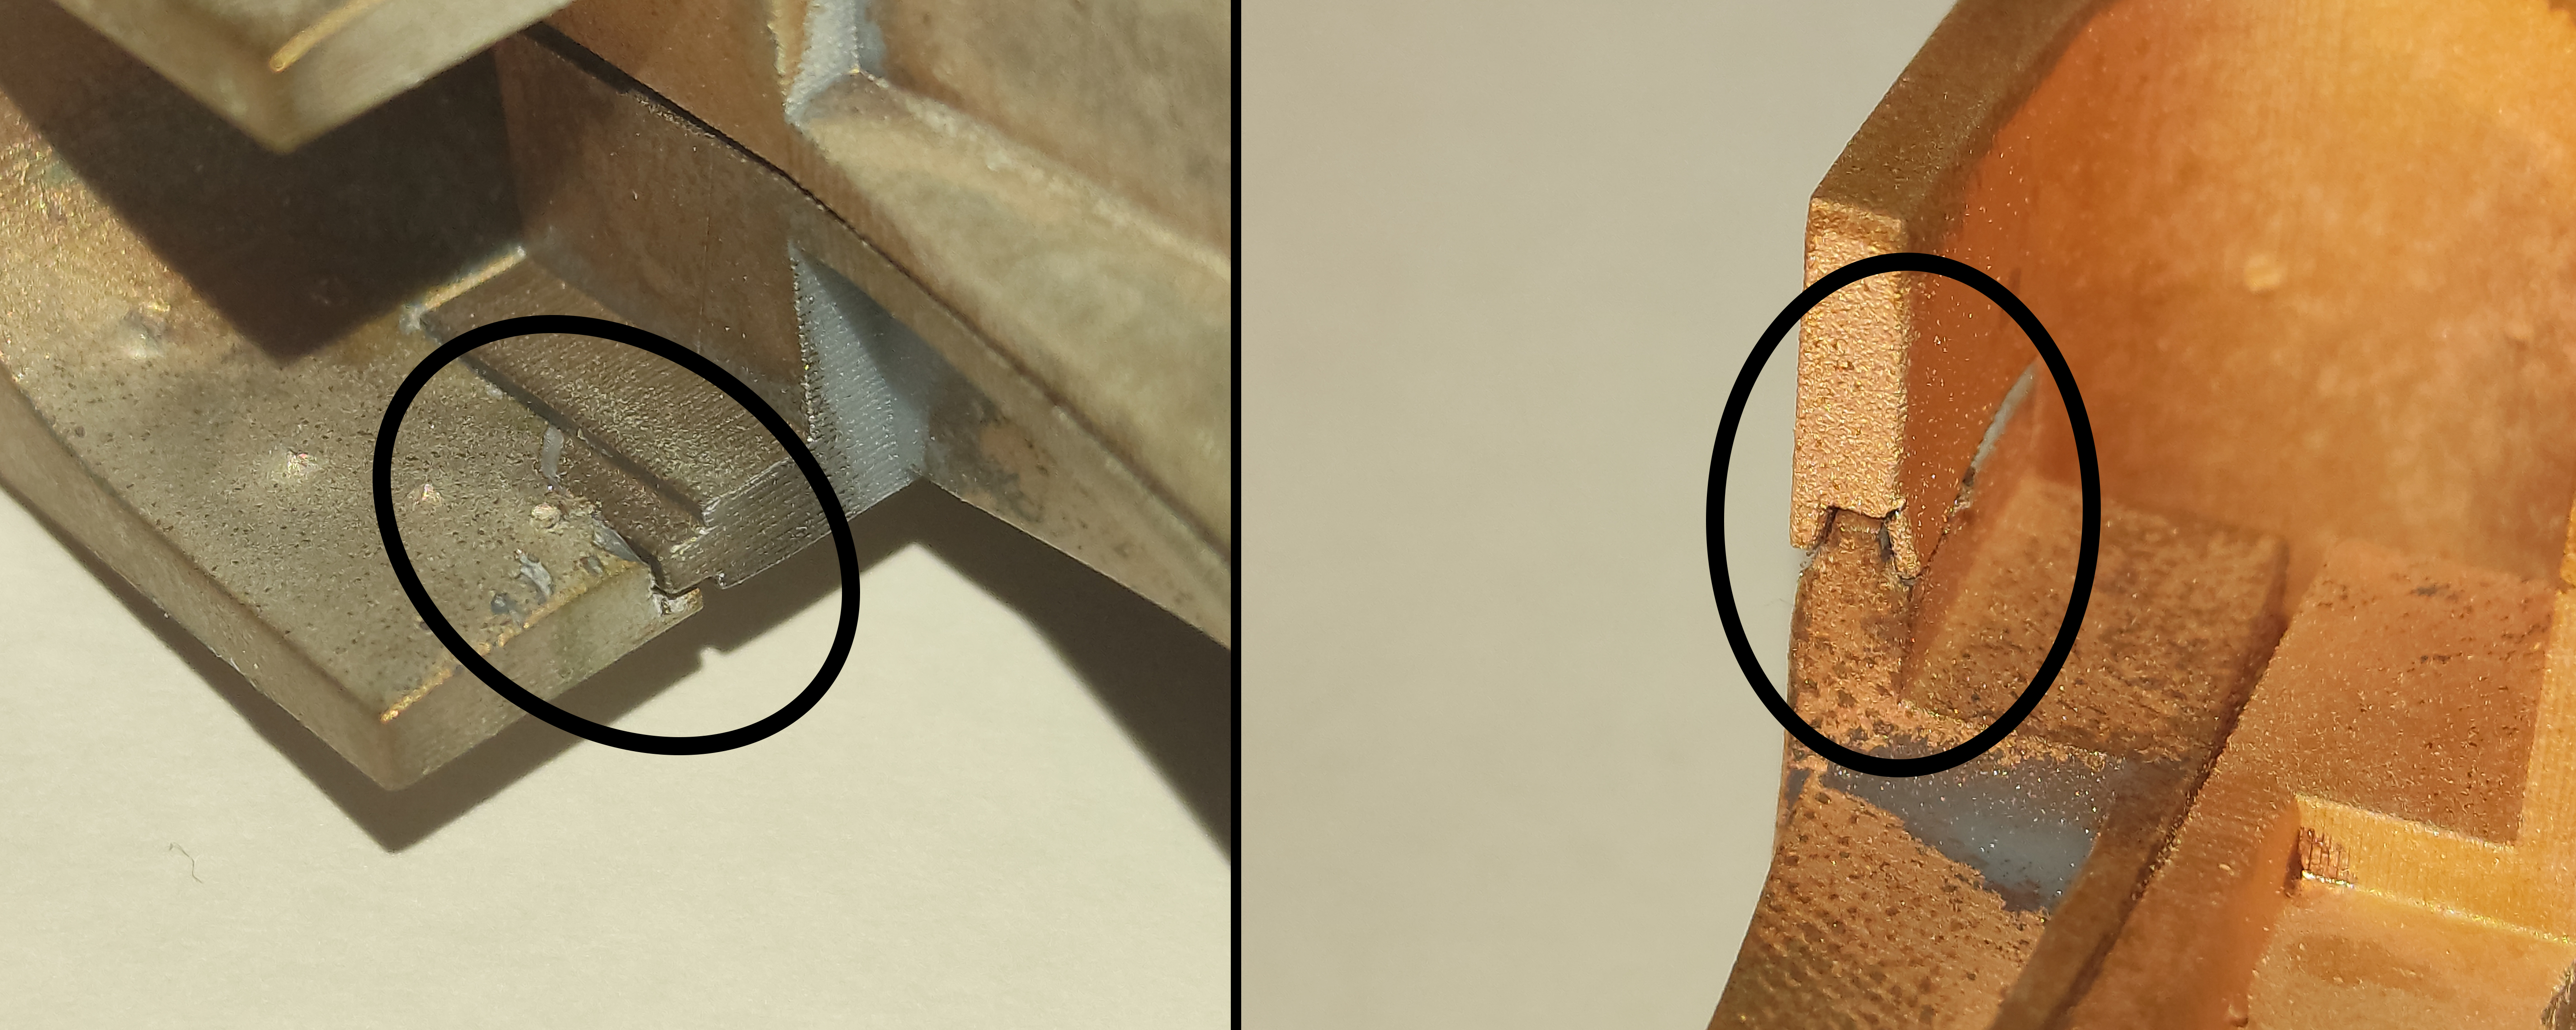
\includegraphics[width=0.75\linewidth]{img/modelos/2025_05_20-Grueso/rupturas.jpg}
    \caption{Rupturas en la conexión vivo-feed del modelo IV.}
    \label{fig:rupturas}
\end{figure}

Para arreglarlo, simplemente se ha modificado la ranura para que sea más gruesa y resistente. Los cambios en el modelo y el resultado de impresión se recogen en la figura \ref{fig:soporteGrueso}.
\begin{figure}[!h]
    \centering
    \includegraphics[width=0.75\linewidth]{img/modelos/2025_05_20-Grueso/SoporteGruesoRes.png}
    \caption{A la izquierda, nuevo modelo para la conexión entre piezas. A la derecha, resultado de impresión.}
    \label{fig:soporteGrueso}
\end{figure}

El resultado es una unión mucho más firme que la anterior, ya que su grosor es aproximadamente el cuádruple. El montaje es mucho más cómodo ahora ya que la holgura de la unión, que era de 0.1 mm, se ha aumentado a 0.4 mm para evitar problemas como los de la figura \ref{fig:rupturas} sin sacrificar estabilidad en dicha unión. 
\begin{figure}[!h]
    \centering
    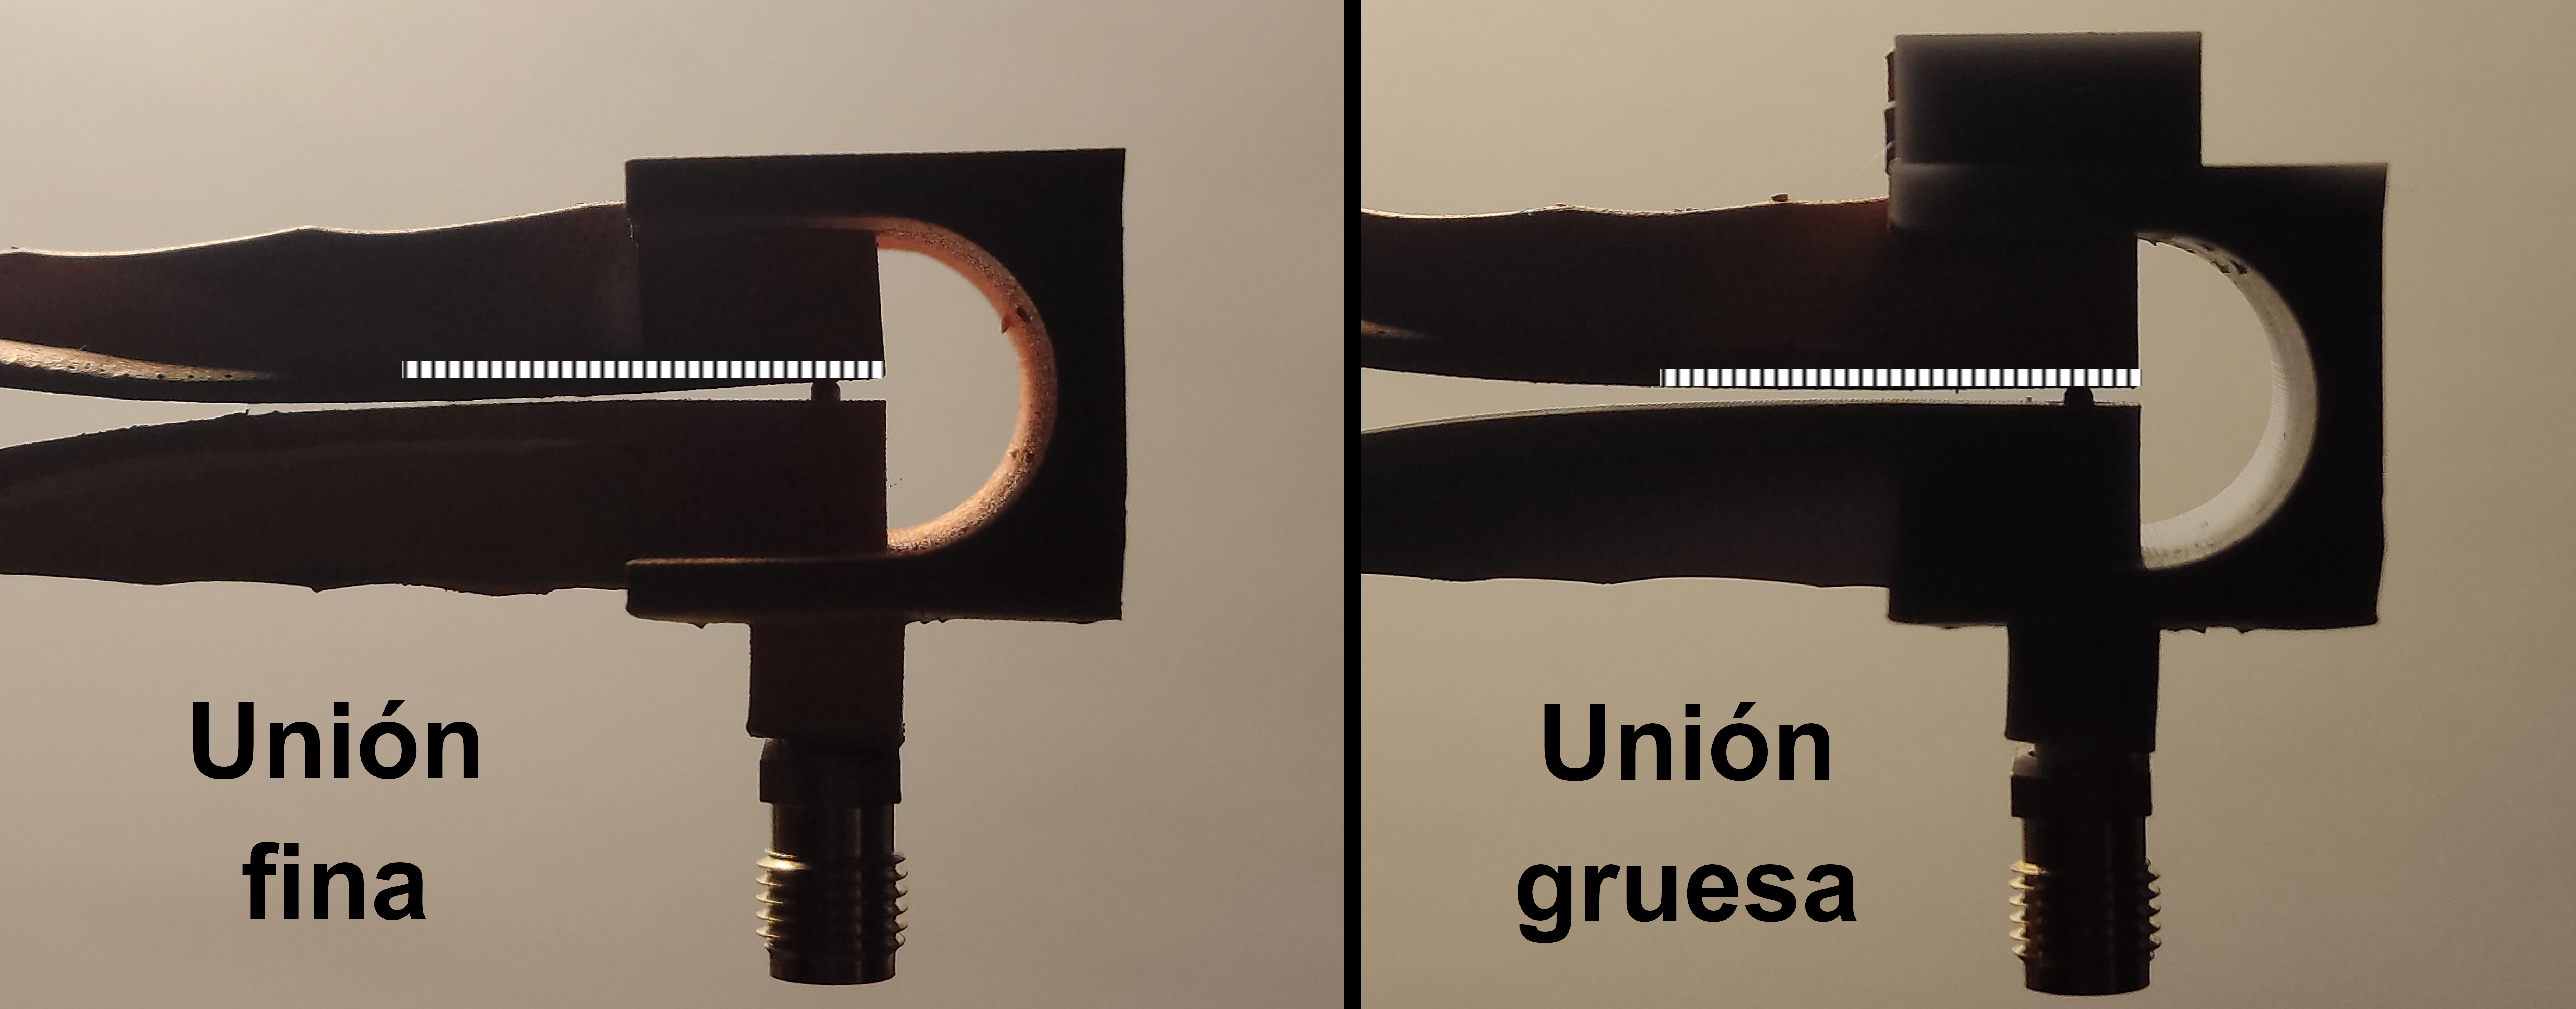
\includegraphics[width=\linewidth]{img/modelos/2025_05_20-Grueso/perfil.jpg}
    \vspace{-0.5cm}
    \caption{Comparación entre los perfiles para la primera unión (fina) y la nueva (gruesa).}
    \label{fig:noParalelo}
\end{figure}

De hecho, esta nueva unión también presenta una mejora muy importante: con la unión gruesa las placas son perfectamente paralelas en el tramo inicial, tal y como fueron diseñadas, mientras que con la unión fina la placa superior no tiene el soporte necesario, por lo que se dobla hacia abajo y las placas se acercan cuando deberían estar alejándose. Esto se aprecia muy bien en la figura \ref{fig:noParalelo}, donde se ha añadido una línea rayada como referencia. Como ya se ha comentado, lo anterior es muy importante ya que la distancia entre las placas debe cumplir la ecuación \ref{eq:d(z)} para que la impedancia de la línea se adapte a la del vacío de forma gradual y la transferencia de potencia sea máxima.


%%%%%%%%%%%%%%%%%%%%%%%%%%%%%%%%%%%%%%%%%%%%%%%%%%%%%%%%%%%%%%%%%%%%%%%%%%%%%%%%
\subsection{Impresión 3D}

% Distintos métodos de impresión -> Fotos de filamento -> agradecimientos -> Decir que se ha optado por impresión en resina -> Fotos + explicación resina

En esta subsección se explicará el funcionamiento de la impresora de resina y la forma de operarla. Como ya se ha explicado, se han hecho pruebas de impresión mediante diferentes impresoras 3D para comparar sus resultados.
\begin{figure}[!h]
    \centering
    \includegraphics[width=\linewidth]{img/fotos/filamento.jpg}
    \vspace{-0.5cm}
    \caption{Arriba a la izquierda: fotos de la antena impresa en Bibliomaker mediante Ender 3 PRO. Arriba a la derecha: fotos de la antena impresa por Federico Coca mediante Prusa i3. Abajo: comparación de los resultados de distintas impresoras.}
    \label{fig:filamento}
\end{figure}

Agradezco de nuevo al personal de Bibliomaker de la Facultad de Ciencias por darme acceso a sus impresoras (fig. \ref{fig:filamento}, arriba a la izquierda) y a Federico Coca por imprimir una antena para este proyecto (fig. \ref{fig:filamento}, arriba a la derecha).\\

Aunque en general ambos resultados usando filamento son buenos, requieren algunos pasos extra de posprocesado para alcanzar la calidad de las impresiones en resina (ver fig. \ref{fig:filamento}), por lo que se usará la impresora de resina para simplificar el proceso. A continuación se hablará más en profundidad acerca de esta última.\\

El funcionamiento de la impresora de resina se basa en la fotopolimerización, un proceso por el cual se solidifica una resina líquida al iluminarla con luz UV. Para ello, se vierte la resina en un tanque con fondo transparente bajo el que se encuentra un dispositivo emisor de luz UV. Al iluminarse, una capa de resina se solidifica con la forma deseada y queda adherida a una plataforma de construcción que está sumergida en la resina. Tras esto, la plataforma se eleva ligeramente, llevándose consigo la capa anterior y dejando que más resina líquida ocupe su lugar para así repetir el proceso capa a capa hasta crear el objeto deseado.\\

En cuanto a su manejo, el primer paso es asegurarse de que no quedan residuos de resina en ninguna pieza. Esto es crítico para el resultado ya que cualquier mancha en el vidrio o superficie exterior del tanque pueden bloquear la luz y, por tanto, evitar la fotopolimerización en ciertas direcciones. Habiendo comprobado esto, el siguiente paso es montar el tanque y la plataforma y asegurarlos mediante sus tornillos (ver fig. \ref{fig:impresoraResina1}).
\begin{figure}[!h]
    \centering
    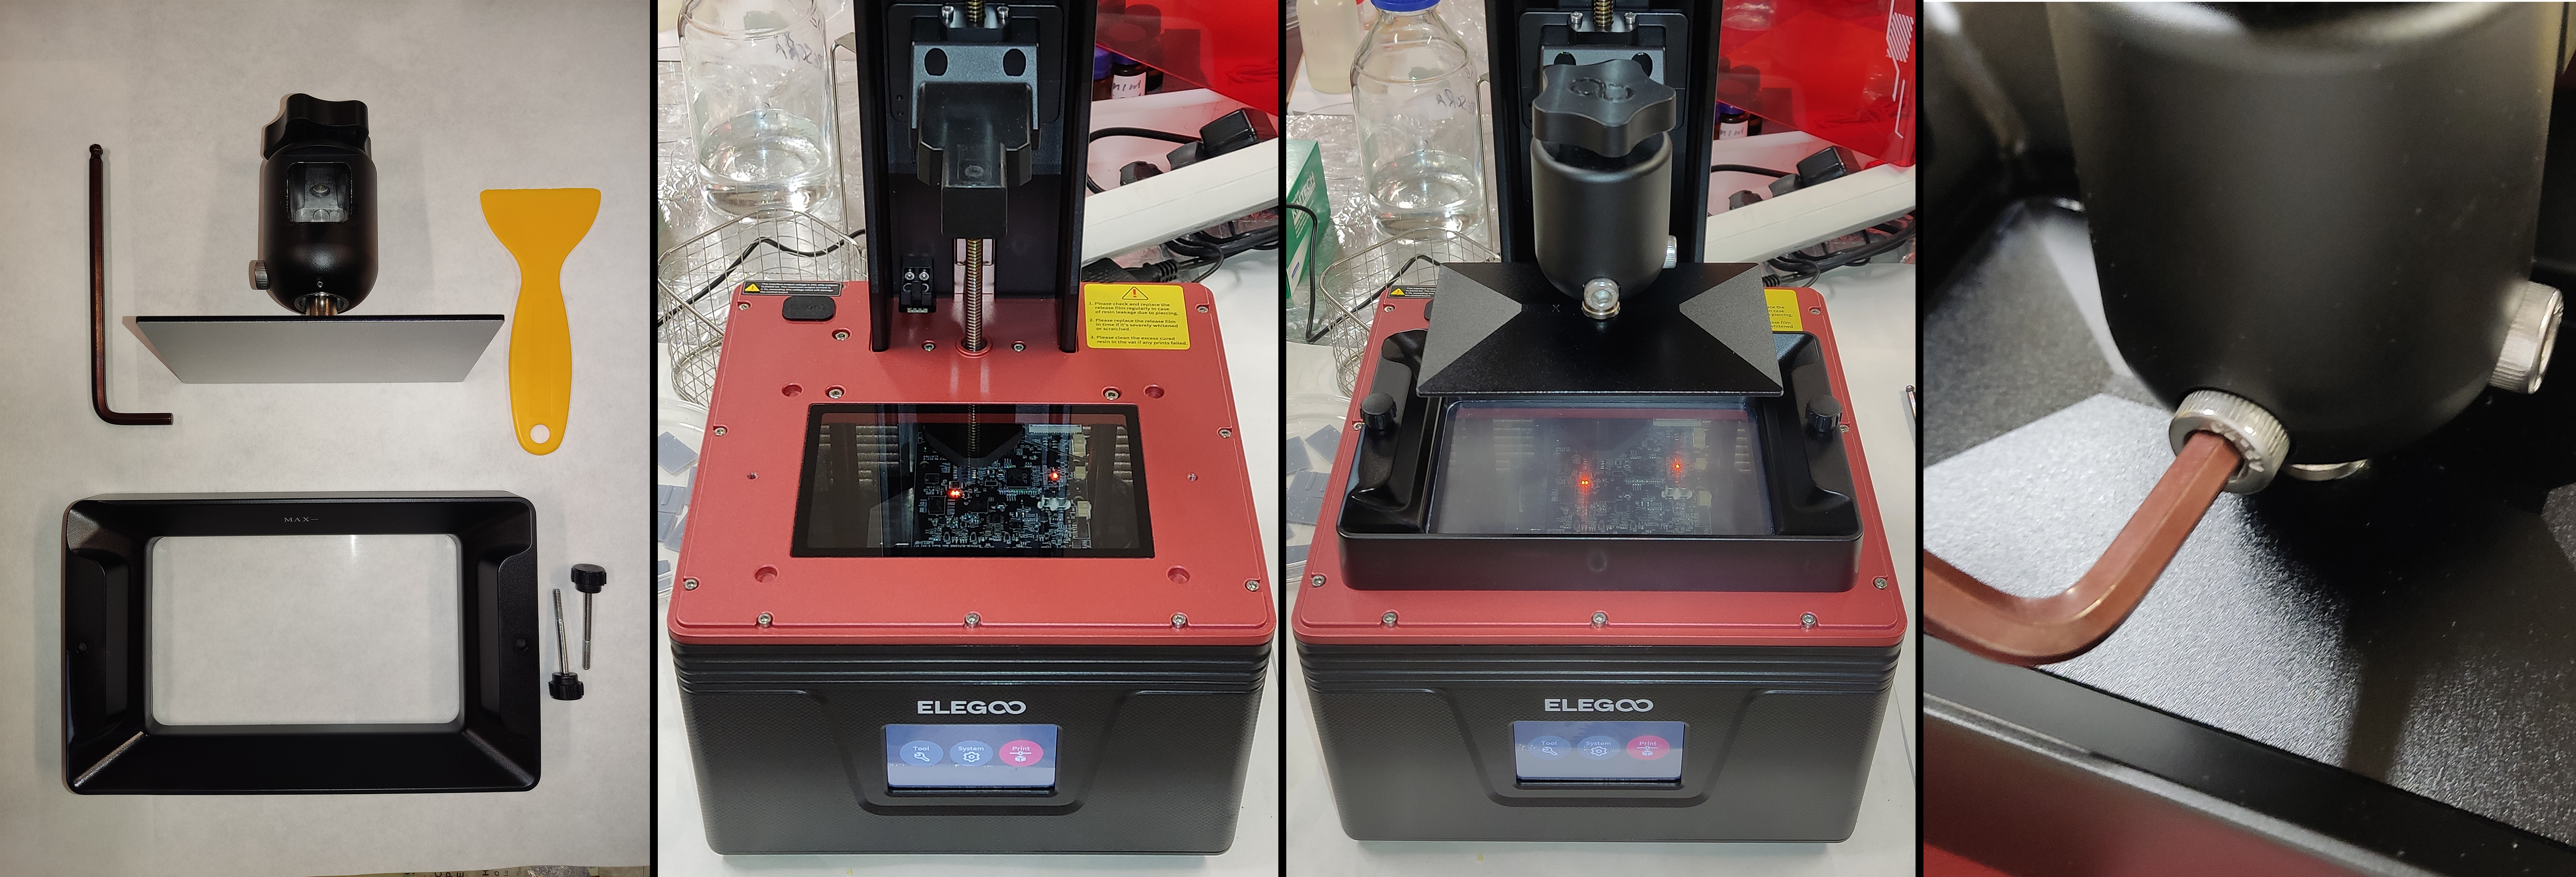
\includegraphics[width=\linewidth]{img/impresionResina/resina1.jpg}
    \vspace{-0.65cm}
    \caption{Elementos y primeros pasos en la preparación de la impresora.}
    \label{fig:impresoraResina1}
\end{figure}

Lo siguiente es usar la llave allen para liberar el movimiento de la plataforma. Luego, se enciende la impresora y se usan los controles de la pantalla táctil para bajar la plataforma completamente. Una vez abajo, se alinea con los bordes del tanque y se vuelve a usar la llave Allen para fijar su posición (fig. \ref{fig:impresoraResina1}). Tras esto, se eleva la plataforma 0.01 mm y se establece su origen en esa posición. Finalmente, el último paso antes de la impresión es subir la plataforma para tener hueco y verter la resina hasta la marca que hay en el tanque y colocar la tapa de la impresora. Hecho esto, se usa la pantalla táctil de la impresora para comenzar la impresión.
\begin{figure}
    \centering
    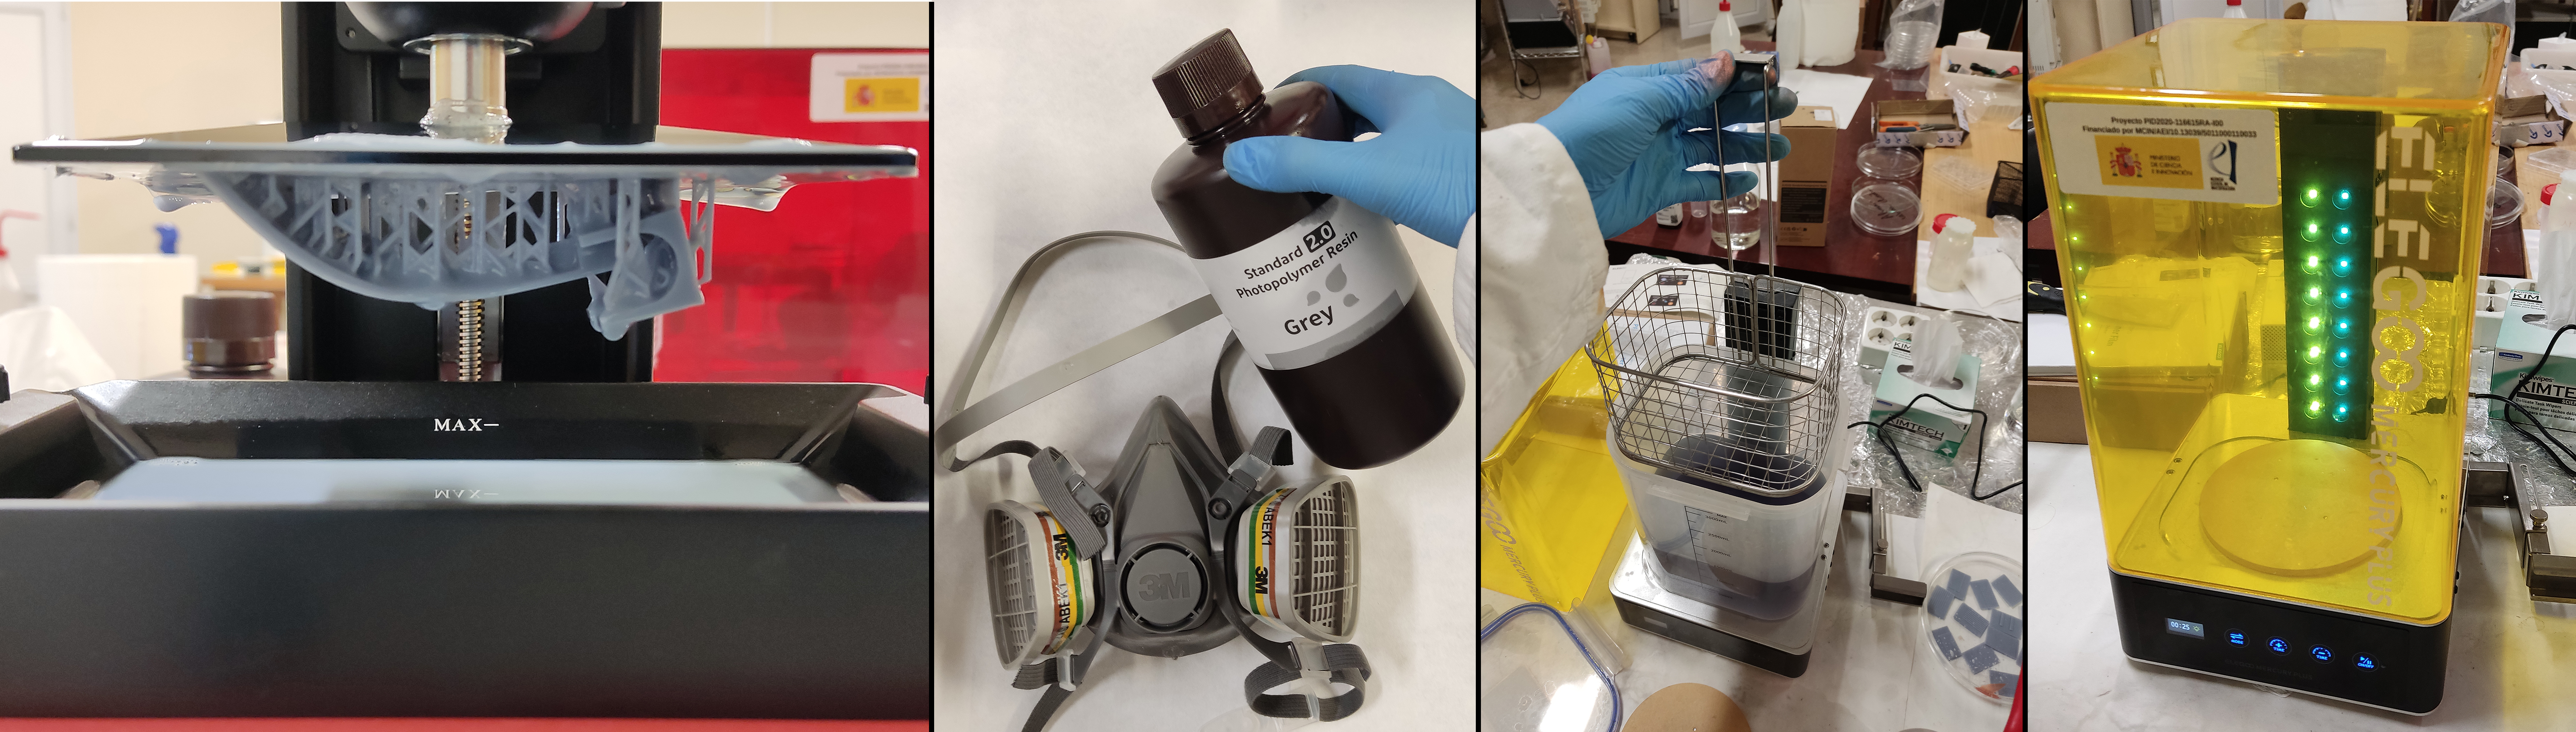
\includegraphics[width=\linewidth]{img/impresionResina/resina2.jpg}
    \vspace{-0.65cm}
    \caption{Fotos de la pieza recién impresa, de la máscara y resina utilizadas y de la estación de lavado y curado.}
    \label{fig:impresoraResina2}
\end{figure}

Cuando ha terminado la impresión (unas 2 horas y 20 minutos en el caso de la pieza más grande de la antena), queda la pieza pegada en la plataforma como se ve en la figura \ref{fig:impresoraResina2} izquierda. Usando una espátula de plástico para no dañar la superficie de la plataforma, se despega la pieza junto con sus soportes de impresión. Después, se introduce en la cesta metálica de la estación de lavado y curado y se sumerge. Se deja lavando durante unos 5 minutos y luego se lava la pieza con alcohol isopropílico y se seca usando aire a presión. Por último, en la estación de lavado y curado se retira el recipiente y se coloca la plataforma circular, sobre la que se dejará la pieza curando durante 7 minutos. Hecho todo esto, ya solo falta quitar los soportes de la pieza y está lista.\\

Durante este proceso se debe llevar la máscara siempre que haya resina líquida. Por otro lado, hay que filtrar y almacenar la resina líquida que ha sobrado en el tanque en un recipiente opaco o que se guarde en un lugar oscuro. También se deben limpiar los restos de resina tanto del tanque como de la plataforma y la espátula, desechando los restos en contenedores cerrados para contener los vapores de la resina líquida.


%%%%%%%%%%%%%%%%%%%%%%%%%%%%%%%%%%%%%%%%%%%%%%%%%%%%%%%%%%%%%%%%%%%%%%%%%%%%%%%%
\subsection{Metalizado de la antena}

\begin{wrapfigure}{r}{5cm}
    \vspace{-1.6cm}
    \includegraphics[width=0.9\linewidth]{img/Metalizado/esquemaElectrolisis.png}
    \vspace{-0.2cm}
    \caption{Esquema de la celda electrolítica.}
    \label{fig:esquemaElectrolisis}
\end{wrapfigure}
Tras la impresión 3D, es necesario metalizar la antena para que sea conductora y pueda emitir o recibir señales. Para ello se ha optado por la técnica de electrodeposición o electroplating, que consiste en utilizar la pieza que queremos metalizar como cátodo en una celda electrolítica (fig. \ref{fig:esquemaElectrolisis}).\\

En los primeros ensayos se usó como electrolito una disolución de CuCl$_2$ con una concentración de 100 g/L en HCl al 20\%. Cuando se conecta la fuente de tensión y se sumergen el ánodo y cátodo, iones de cobre pasan desde el ánodo de cobre a la disolución y viajan hacia el cátodo, donde se depositan en la superficie y crean una capa.
\begin{figure}[!h]
    \centering
    \includegraphics[width=0.9\linewidth]{img/Metalizado/pinturaCobre.jpg}
    \vspace{-0.2cm}
    \caption{Pieza pintada con pintura de cobre y medidas de resistencia antes y después del electroplating.}
    \label{fig:pinturaCobre}
\end{figure}

Antes de sumergir la antena en el baño electrolítico es necesario darle varias capas de pintura de cobre. Esta pintura no conduce bien cuando se mide con un multímetro (ver fig. \ref{fig:pinturaCobre}) debido a que las partículas de cobre se encuentran separadas por el aglutintante y, en general, dan lugar a una red no percolante. Esto cambia cuando se sumerge en el electrolito ya que al ir desapareciendo el aglutintante y depositándose más partículas de cobre, la conductividad aumenta rápidamente. Esto hace que cambie el color también, ya que inicialmente las partículas de cobre están aisladas del aire, mientras que tras el metalizado el cobre entra en contacto con el aire y se oxida rápidamente, dando lugar a la diferencia entre superficies que se ve en la figura \ref{fig:pinturaCobre}.\\

En cuanto al procedimiento, es fundamental limpiar la pieza adecuadamente para que la adherencia de la pintura sea máxima. Para ello se ha lavado usando detergente Micro-90. Tras esto, se seca la pieza con aire comprimido. Desde este punto hasta que se termine de metalizar, todo el procedimiento se realizará en una campana extractora para evitar respirar el spray de cobre y los vapores del electrolito. Ya en la campana, se aplican finas capas de pintura de cobre en spray desde unos 30 cm, sosteniéndola con pinzas y dejando secar al menos 5 minutos.\\

Una vez se han aplicado varias capas de pintura de cobre, se usa una pinza cocodrilo para conectar la pieza que queremos metalizar a la fuente. Por la forma en la que funciona el electroplating y, dado que la pintura presenta alta resistencia, el metalizado es mucho más eficiente en la región más cercana a la pinza, por lo que hay que ir cambiando la posición de la pinza constantemente para intentar que la metalización sea uniforme por toda la superficie.\\

Dado que no se disponía de mucho volumen de electrolito, se ha usado un vaso relativamente pequeño para que la pieza pueda quedar sumergida completamente. Esto da lugar a un resultado algo peor, ya que normalmente el electroplating se realiza colocando la pieza en el centro de un recipiente amplio y, rodeando dicha pieza, se colocan una o varias placas de cobre para que la deposición de los iones se realice desde todas las direcciones dando lugar a un metalizado más homogéneo. Por el contrario, para las primeras pruebas de metalizado se ha usado como ánodo la punta de un cable de cobre en lugar de las placas por la falta de espacio.\\

Los resultados de estas primeras pruebas de metalizado se recogen en la figura \ref{fig:metalizado1}.
\begin{figure}[!h]
    \centering
    
\includegraphics[width=\linewidth]{img/Metalizado/metal1.jpg}
    \vspace{-0.5cm}
    \caption{Resultados con el primer método de metalizado.}
    \label{fig:metalizado1}
\end{figure}

Como se ve en la figura \ref{fig:metalizado1} (izq), se ha realizado una prueba de metalizado para una antena impresa mediante una impresora de filamento Prusa i3, de mayor precisión que la Ender 3 PRO. El resultado es bastante mejor que el de esta última ya que no presenta errores de impresión, las líneas de capa son mucho menos visibles y la superficie más suave en general. No obstante, el resultado sigue siendo notablemente peor que en las impresiones de resina, y la pintura de cobre y el metalizado muestran problemas de adhesión que se hacen más visibles por las esquinas. Todo esto se puede mejorar aplicando el posprocesado adecuado a las piezas antes de pintarlas y metalizarlas (lijado, imprimación, ...), pero se ha optado por seguir usando resina ya que se obtienen resultados mejores y de manera más sencilla.\\

Tanto la pieza central como la derecha de la figura \ref{fig:metalizado1} se muestran sin la mitad superior de la antena para ver mejor la superficie pero estas también se metalizaron, siendo en total 6 piezas metalizadas mediante el electrolito de CuCl$_2$. En las distintas pruebas se usaron diferentes valores de corriente y voltaje y se sumergieron las piezas entre 2 y 15 minutos según la prueba para ver los efectos del tiempo en la conductividad.

En los mejores casos, al sacar la pieza del electrolito y rápidamente usar un multímetro para medir la resistencia entre las puntas exteriores de la placa ((a) y (b) en la fig. \ref{fig:metalizado1}) se han obtenido valores del orden de $\sim$10 $\Omega$, mientras que al medirla entre una punta y el bloque del feed (c) la resistencia es del orden de M$\Omega$ en los casos en que el multímetro era capaz de medirla. 

Estas resistencias aumentaban rápidamente al volver a medirlas pasados pocos minutos, quedando ambas fuera del rango del multímetro en todas las pruebas. En este punto ya se han formado los patrones de oxidación en la superficie de la pieza y se ha evaporado la película de electrolito que cubría su superficie. Probablemente lo que permite que se midan resistencias más bajas es la capa de electrolito (que es conductor) que aún quedaba en la superficie, por lo que cuando esta se evapora y rápidamente se oxida la pieza la resistencia aumenta drásticamente y deja de ser conductora. 

Por motivos que se discutirán un poco más adelante, se estaban usando corrientes tan bajas ($<100$ mA en todos los casos) que los cambios en la tensión de la fuente prácticamente no afectaban al resultado final. De esta manera, el único parámetro que ha resultado relevante en estos ensayos es el tiempo de metalizado, dando resultados ligeramente mejores cuanto mayor es el mismo.\\

Para intentar mejorar los resultados, se probará un método de metalizado algo diferente. A continuación se explican los cambios, basados en las recomendaciones de Hendrik Vogelpohl en su canal de YouTube dedicado a electroplating \cite{hen3drik}.
\begin{figure}[!h]
    \centering
    \includegraphics[width=0.9\linewidth]{img/Metalizado/metal2.jpg}
    \vspace{-0.1cm}
    \caption{De izquierda a derecha: electrolitos usados en cada método, tubo de cobre usado como ánodo y pieza enrollada en cable como cátodo.}
    \label{fig:metalizado2}
\end{figure}

Para empezar, se usa un electrolito diferente, hecho con CuSO$_4$ en 125 g/L y H$_2$SO$_4$ en 60 g/L (ver fig. \ref{fig:metalizado2} izquierda), para comprobar si mejora la deposición de cobre y conductividad.\\

También se ha optado por usar como ánodo un tubo de cobre (fig. \ref{fig:metalizado2} central) en lugar de un cable. Se ha hecho esto porque se han usado cables multifilares y durante la electrólisis, al donar cobre al electrolito van perdiendo material y volviéndose más finos, por lo que acaban rompiéndose por distintos lugares y dejando caer grandes trozos de hilo al fondo del recipiente que dejan de formar parte del ánodo, por lo que hay que permanecer atento para regular manualmente la fuente y que la corriente y voltaje sean los deseados siempre. Por otro lado, el tubo de cobre tiene una estructura maciza y su tamaño no cambia significativamente en el transcurso del metalizado, por lo que la tensión y corriente suministradas por la fuente permanecerán constantes. De este modo, ya no es necesario vigilar todo el proceso, por lo que es más plausible metalizar durante varias horas y así crear recubrimientos más gruesos.\\

Por el lado del cátodo, en lugar de usar la pinza de cocodrilo se ha usado un cable para enrollar la pieza (fig. \ref{fig:metalizado2} derecha) y que la deposición sea más uniforme. Esto se hace para evitar que la deposición se focalice en la pinza, ya que habría que ir cambiando su posición continuamente. Gracias a esto y a lo que se ha comentado anteriormente, es más cómodo metalizar durante largos períodos. El único inconveniente es que al enrollar la pieza hay que evitar un contacto muy estrecho entre el cable y la pieza porque el recubrimiento acaba conectando el cable con la pieza y se desprende al separarlos (fig. \ref{fig:desperfectosMetalizado} izquierda).\\

En cuanto a la fuente, se ha determinado su configuración mediante las leyes de Faraday de la electrólisis \cite{walsh}, con las ecuaciones
\begin{equation}\label{eq:espesor}
    \begin{cases}
        m = \frac{ItM}{nF}\\
        s = \frac{m}{\rho A}
    \end{cases} \Rightarrow
    s = \frac{ItM}{n\rho FA}
\end{equation}
donde $m$ es la masa depositada, $I$ la corriente, $M=63.35$ g/mol la masa molar del cobre, $n$ la valencia del cobre en la reacción (+2 al ser Cu$^{2+}$), $F$ la constante de Faraday, $s$ el espesor de la capa de cobre, $\rho=8.96$ g/cm su densidad y $A\simeq100$ cm$^2$ el área de la pieza que se metaliza.\\

Mediante la ecuación \ref{eq:espesor} se puede elegir el espesor deseado para la capa de cobre y el tiempo que durará el proceso y entonces despejar la corriente $I$ que debe suministrar la fuente. Lo ideal es encontrar un equilibrio entre estos parámetros ya que si, por ejemplo, se elije un tiempo muy corto de metalización, la corriente necesaria para alcanzar cierto espesor $s$ será muy alta. Al llevar esto a cabo el resultado es un burbujeo durante la deposición que acaba dando lugar a una superficie irregular relativamente frágil de metal \cite{hen3drik}. Por ello se ha decidido aumentar el tiempo de metalizado a, al menos, dos horas.

Este tiempo es importante, pero cabe destacar que no ha sido el factor crítico para la mejora de resultados que se comentará más adelante ya que usando todos estos cambios se ha hecho una prueba extrayendo la pieza del baño electrolítico tras 10 minutos y las resistencias ya eran menores a 1 $\Omega$ entre sus extremos\footnote{Aunque se siguen usando de aquí en adelante para comparar, los multímetros como el que se ha usado dejan de dar mediciones correctas para resistencias menores a unos 2 $\Omega$. Para conocer los valores reales habría que usar el método de Kelvin de medición a cuatro puntas.}.

Se ha elegido un grosor de $17$ micras y una duración de dos horas por lo que, según la ecuación \ref{eq:espesor}, la corriente que suministra la fuente debe ser
\begin{equation*}
    I = \frac{sn\rho FA}{tM} = \frac{0.0017\cdot2\cdot8.96\cdot96485\cdot100}{7200\cdot63.55} \simeq 0.642 \text{ A.}
\end{equation*}
\vspace{-0.6cm}
\begin{figure}[!h]
    \centering
    \includegraphics[width=\linewidth]{img/Metalizado/metalizadoCampana.jpg}
    \vspace{-0.7cm}
    \caption{Puesta a cabo experimental con los cambios en el procedimiento.}
    \label{fig:campana}
\end{figure}

Tras estos cambios, la realización experimental es la que se recoge en las fotos de la figura \ref{fig:campana}, y se obtienen como resultado las piezas de la figura \ref{fig:metalizado3}. En cuanto a su conductividad, ambas presentan resistencias de menos de 0.5 $\Omega$ medidas de extremo a extremo, y menores a 1.5 $\Omega$ entre cualquiera de los terminales del conector y el extremo de las placas, probablemente debido a que el contacto entre la antena y el conector es puramente mecánico y depende de la presión con la que se unen y la calidad del metalizado y su superficie en el punto de contacto. A pesar de esto, este segundo método presenta una mejora muy significativa respecto al primero al observar las propiedades eléctricas.
\begin{figure}[!h]
    \centering
    \includegraphics[width=0.9\linewidth]{img/Metalizado/resultadosMetalizado2.jpg}
    \caption{Resultados del metalizado tras los cambios propuestos.}
    \label{fig:metalizado3}
\end{figure}

El principal problema de la antena ahora es que es relativamente frágil, ya que podría rayarse o desprenderse la capa de cobre. Además, es sensible al contacto con los dedos y quedan marcas bastante visibles (fig. \ref{fig:desperfectosMetalizado} central), al igual que en las partes que no se metalizan debido a burbujas de aire adheridas a la superficie de la pieza (fig. \ref{fig:desperfectosMetalizado} derecha), por lo que es recomendable agitarla al introducirla en el baño electrolítico para que se desprendan estas burbujas.
\begin{figure}[!h]
    \centering
    
\includegraphics[width=\linewidth]{img/Metalizado/desperfectosMetalizado.jpg}
    \vspace{-0.5cm}
    \caption{Desperfectos en el metalizado.}
    \label{fig:desperfectosMetalizado}
\end{figure}


%%%%%%%%%%%%%%%%%%%%%%%%%%%%%%%%%%%%%%%%%%%%%%%%%%%%%%%%%%%%%%%%%%%%%%%%%%%%%%%%
%%%%%%%%%%%%%%%%%%%%%%%%%%%%%%%%%%%%%%%%%%%%%%%%%%%%%%%%%%%%%%%%%%%%%%%%%%%%%%%%
\section{Resultados}

En esta sección se explicará cómo se han obtenido los distintos resultados del análisis de la antena, por un lado mediante simulación y por otro usando un VNA para medir la antena que se ha construido. Luego, se compararán y se discutirán las razones de sus similitudes y diferencias.

%%%%%%%%%%%%%%%%%%%%%%%%%%%%%%%%%%%%%%%%%%%%%%%%%%%%%%%%%%%%%%%%%%%%%%%%%%%%%%%%
\subsection{Resultados de la simulación}

En primer lugar me gustaría agradecer de nuevo al equipo de Elemwave por darme acceso a su software de simulación \textit{Elemwave Workbench} y por su ayuda a lo largo de todo el proceso. Este software se instala sobre FreeCad, de manera que se usan todas sus herramientas de forma conjunta.

El objetivo de esta simulación es obtener una serie de resultados que luego se compararán con los experimentales.\\

Tras introducir el modelo de la antena (.stl) en el simulador, se ha cerrado el hueco del conector ya que la entrada se generará de una forma diferente que se explicará más adelante. A continuación se crea el \textit{mesh} o mallado de la antena. Este paso es fundamental ya que transforma el modelo 3D continuo de la antena en uno discreto formado por cubos (celdas de Yee), que es con lo que trabajará el simulador. 

Se usa el método FDTD (diferencias finitas en el dominio del tiempo), que es muy preciso y, al trabajar en el dominio del tiempo, puede calcular la respuesta impulso del sistema \cite{FDTD}. Esto hace que se puedan estudiar múltiples frecuencias muy eficientemente ya que el impulso ideal contiene todas las frecuencias al ser la transformada de Fourier de la Delta de Dirac la función constante unidad.\\
\begin{figure}[!h]
    \centering
    \includegraphics[width=\linewidth]{img/simulación/mallado.jpg}
    \vspace{-0.5cm}
    \caption{a) Antena (transparente) superpuesta al mallado (rojo). b) Detalle del modelo de la antena y la malla superpuestos. c) y d) Perfil de la antena antes y después del mallado, con cuadrícula superpuesta.}
    \label{fig:mallado}
\end{figure}

En la figura \ref{fig:mallado} b) se aprecia la discretización del modelo, y en d) se distingue cómo el mallado se construye en términos del la cuadrícula que hemos definido. Las celdas de esta cuadrícula deben ser lo bastante pequeñas en comparación de la longitud de onda más corta con la que se quiere simular, típicamente $\lambda/20$. En nuestro caso, gracias a los resultados de Mallahzadeh \cite{tem_horn} tenemos como objetivo una frecuencia máxima de 14 GHz, por lo que las celdas tienen dimensiones máximas de $0.02142/20 = 0.001$ m. Como resultado, la simulación está formada por unos 10 millones de celdas.\\

El motivo por el que se ha cerrado el hueco del conector es la forma en la que se simulará la fuente. Se definirá una línea que conecta las dos placas pasando donde lo haría el vivo del conector, como se ve en la figura \ref{fig:simCable} central. En el centro de dicho cable se colocará una fuente con resistencia de 50 $\Omega$ (igual que la impedancia característica de la línea de transmisión) en serie y también las sondas que medirán los valores de $i$ y $v$ en cada paso temporal. La fuente emite un pulso de muy corta duración temporal (0.15 ns) que se ve en la figura \ref{fig:simCable} izquierda.
\begin{figure}[!h]
    \centering
    \includegraphics[width=\linewidth]{img/simulación/cableSim.jpg}
    \vspace{-0.5cm}
    \caption{Izquierda: Pulso de la fuente, con voltaje en V y tiempo en s. Centro: Detalle del cable-fuente. Derecha: Direcciones en las que se guardan las medidas de campo lejano.}
    \label{fig:simCable}
\end{figure}

Dado que la simulación no se puede realizar para el espacio abierto, se define una región que contiene a la antena en su totalidad de manera que las ondas se simulan en su interior y, cuando alcanzan dicha frontera, son absorbidas, imitando el efecto del espacio abierto. Para ello, se han usado condiciones de frontera PML (Perfectly Matched Layer).

Conociendo los valores de los campos en la frontera, el simulador calcula cuál será su distribución en campo lejano. Para estudiar el patrón de emisión se han colocado sondas de campo lejano a lo largo de la dirección $\theta$ (fig. \ref{fig:simCable} derecha).

\begin{figure}[!h]
    \centering
    \includegraphics[width=\linewidth]{img/simulación/patronRadiacion.png}
    \vspace{-0.5cm}
    \caption{Patrones de emisión: módulo del campo eléctrico en función de $\theta$ para distintas frecuencias (normalizado).}
    \label{fig:patronEmision}
\end{figure}
Las medidas de las sondas para diferentes frecuencias dan como resultado los patrones de emisión de la figura \ref{fig:patronEmision}. Para 1 GHz, la longitud de onda es de unos 30 cm, por lo que el tamaño eléctrico de la antena es pequeño (unos 8 cm) y su capacidad para enfocar la emisión en cierta dirección se reduce mucho. A medida que aumenta la frecuencia, la longitud de onda disminuye y la geometría de las distintas partes de la antena empieza a influir en el patrón de emisión de formas que son muy difíciles de predecir sin el uso de simulaciones ya que entran en juego modos de propagación de orden superior e interactúan con elementos como las uniones de piezas o los bordes de formas complejas. A partir de una frecuencia de unos 3 GHz, la antena es muy directiva en la dirección deseada, pero si se deseara usarla para emitir frecuencias más bajas, sería necesario reescalar sus dimensiones para agrandarla y que tenga un tamaño eléctrico lo bastante grande para dichas frecuencias.\\

El resto de resultados de la simulación se obtienen a partir de dos ficheros diferentes: uno con el voltaje del pulso que emite la fuente en función del tiempo, y otro con la corriente medida por la sonda de la fuente en función del tiempo. 

Se ha realizado una interpolación y extrapolación de los datos del pulso de voltaje para unificar los valores de $i(t)$ y $v(t)$ bajo el mismo paso e intervalo de $t$, como se ve en la gráfica superior derecha de la figura \ref{fig:plotSim}. Esto es importante porque el siguiente paso será cambiar la corriente y el voltaje al dominio de la frecuencia mediante una transformada de Fourier y es necesario que sus datos estén muestreados para los mismos instantes de tiempo y con la misma frecuencia de muestreo para que las operaciones con sus transformadas de Fourier se puedan realizar. 

A continuación, se calcula la transformada de Fourier de $i(t)$ y $v(t)$ para obtener los fasores $I$ y $V$, y luego obtener la impedancia de entrada $Z_{in}=V/I$. Como se ha comentado antes, la fuente lleva una impedancia $Z_s=50$ $\Omega$ y, como la sonda de voltaje está en el generador, mide $Z_{in}=Z_s+Z_L$, por lo que $Z_L=Z_{in}-50$ $\Omega$. En la figura \ref{fig:plotSim} se recogen los resultados para el módulo de $Z_L$ y sus partes real e imaginaria en función del tiempo.

Por último, conocidos los valores de $Z_L$ y $Z_0$ para el rango de frecuencias deseado, se calcula el parámetro $S_{11}$ en decibelios mediante la expresión \ref{eq:S11} y se obtiene como resultado la gráfica inferior derecha de la figura \ref{fig:plotSim}, que se discutirá en secciones posteriores.
\vspace{-0.5cm}
\begin{figure}[!h]
    \centering
    \includegraphics[width=0.99\linewidth]{img/simulación/plotsSim.png}
    \vspace{-0.4cm}
    \caption{Resultados para la impedancia de carga y $S_{11}$ en función de la frecuencia usando la simulación, e interpolación y extrapolación de $V(t)$.}
    \label{fig:plotSim}
\end{figure}


%%%%%%%%%%%%%%%%%%%%%%%%%%%%%%%%%%%%%%%%%%%%%%%%%%%%%%%%%%%%%%%%%%%%%%%%%%%%%%%%
\subsection{Resultados experimentales}

Agradezco de nuevo a Mario Fernández Pantoja por su ayuda para medir los parámetros de la antena mediante VNA.

Se han realizado medidas del parámetro $S_{11}$ de dos antenas diferentes, una con la unión fina y otra con la unión gruesa, como las de la figura \ref{fig:noParalelo}. Ambas se han montado de forma similar, asegurando el conector mediante tornillos y tuercas, pero como en el modelo de unión gruesa la tierra del conector no hacía buen contacto (fig. \ref{fig:contactoAluminio}) se han introducido dos trozos de papel de aluminio doblados varias veces entre la antena y la tierra del conector.
\begin{figure}[!h]
    \centering
    \includegraphics[width=\linewidth]{img/medidasExp/contactoAluminio.jpg}
    \vspace{-0.5cm}
    \caption{De izquierda a derecha: Falta de contacto entre la antena y la tierra del conector, colocación del papel de aluminio, buen contacto gracias al papel de aluminio y resultado final.}
    \label{fig:contactoAluminio}
\end{figure}

Para medir el $S_{11}$ se ha usado el VNA (analizador vectorial de redes) de la figura \ref{fig:VNA} izquierda, un Keysight E5071C. Los datos de $S_{11}$ que se muestran en esa misma figura también se guardan en un archivo para poder tratarlos, de modo que se han guardado para ambas antenas. También permite ver las partes real e imaginaria de la impedancia (fig. \ref{fig:VNA} derecha), que no se han podido guardar directamente en un fichero pero se representarán más adelante usando los datos de $S_{11}$.
\begin{figure}[!h]
    \centering
    \includegraphics[width=\linewidth]{img/medidasExp/VNA.jpg}
    \vspace{-0.5cm}
    \caption{Fotos de la antena conectada al VNA y de las partes real e imaginaria de la impedancia para la antena de unión fina.}
    \label{fig:VNA}
\end{figure}

Los resultados del módulo y fase de $S_{11}$ y partes real e imaginaria para cada antena se recogen en la figura \ref{fig:S11ZExp}. Dado que el VNA guarda los datos en archivos ''.S1P'', se ha usado la librería de Python \textit{scikit-rf} para tratarlos ya que que permite cargar ese tipo de archivos y dispone de funciones para obtener fácilmente las impedancias a partir de ellos \cite{skrf}. 

Para empezar resulta llamativo que, en contra de las previsiones que se hicieron cuando se discutía la construcción de la antena, resulta que el ancho de banda de la antena con el soporte fino es mayor que el de la antena con soporte grueso. En ambos casos aparece un pico negativo (resonancia o impedance matching) muy profundo en torno a 1.58 GHz, es decir, a una media longitud de onda de 9.4 cm, por lo que esta resonancia se corresponde con la longitud del borde exterior de las placas de la antena.

Por otro lado, entre los 3 y los 7 GHz hay una zona más estable en cuanto a impedancias en la que la parte real queda cercana a los 50 $\Omega$ mientras que la imaginaria oscila entre -25 y 50 $\Omega$. En esta región hay tres resonancias, dos de las cuales presentan $|S_{11}|<-10$ dB. Las longitudes para estas resonancias son de 2.45 cm y 3 cm, similares al ancho del soporte del feed o a la longitud de la cresta de las placas. 

Las diferencias en la construcción de cada antena hacen que estos picos, aunque bastante cercanos, no se encuentren en las mismas frecuencias. Para asegurarse de cuáles son las dimensiones responsables de los mismos, lo ideal sería ir añadiendo modificaciones al modelo de la antena gradualmente mientras se estudian estos mismos resultados, ya sea con el simulador o construyéndolas con los procedimientos comentados.
\begin{figure}[!h]
    \centering
    \includegraphics[width=\linewidth]{img/medidasExp/S11Z.png}
    \vspace{-0.5cm}
    \caption{Resultados experimentales de impedancias y $S_{11}$ para las dos antenas.}
    \label{fig:S11ZExp}
\end{figure}


%%%%%%%%%%%%%%%%%%%%%%%%%%%%%%%%%%%%%%%%%%%%%%%%%%%%%%%%%%%%%%%%%%%%%%%%%%%%%%%%
\subsection{Comparación entre resultados}

En la figura \ref{fig:comparacionResultados} se recogen los resultados de $|S_{11}|$ para las medidas experimentales de las antenas mediante el VNA y también el que se ha obtenido mediante la simulación.\\

\begin{figure}[!h]
    \centering
    \includegraphics[width=\linewidth]{img/S11_todos.png}
    \vspace{-0.5cm}
    \caption{$|S_{11}|$ en función de la frecuencia para dos de las antenas que se han construido y para la simulación.}
    \label{fig:comparacionResultados}
\end{figure}
El comportamiento general de las diferentes curvas es muy parecido, con un número similar de resonancias que se encuentran en frecuencias cercanas en la mayoría de los casos, por lo que podemos decir que la simulación es una representación muy adecuada de la antena que se ha construido. No obstante, el hecho de que las diferencias tan pequeñas que puede haber entre las distintas antenas tengan consecuencias en el desplazamiento de las frecuencias de resonancia y en la calidad de dichas resonancias ayuda a ver lo extremadamente sensible que es el diseño de antenas de radiofrecuencia/microondas a los cambios en la geometría ya que, como se ha explicado, los elementos de estas antenas tienen tamaños del orden de las longitudes de onda con las que se trabaja.\\

La diferencia más significativa entre el resultado simulado y los del VNA es el ancho de banda operativo y las frecuencias en las que se da. Por un lado, según la simulación habrá una resonancia en 3.14 GHz con ancho de banda $B=0.53$ GHz. Por otro lado, para las antenas reales esa resonancia es muy pequeña ($\sim-9.4$ dB) y aparece para frecuencias más altas, lo que podría indicar que las dimensiones eléctricas efectivas de la parte de la antena en la que sucede esa resonancia son mayores en la simulación que en las antenas reales, ya sea por su tamaño físico, por imperfecciones geométricas o por cambios en las propiedades de los materiales. Cambios de grosor en la impresión y metalizado, impurezas en el electrolito o irregularidades en la superficie son algunos de los posibles factores que pueden influir en esto además, por supuesto, de la posición de otros elementos del montaje como tornillos o conector que no se han simulado.\\

Para que los resultados sean aún más representativos de la antena real, en la simulación se debería aumentar la resolución del mallado para conseguir una curva más suave en los bordes de la antena y el reflector (fig. \ref{fig:mallado} b) y d)), y las medidas del VNA se deberían realizar varias veces, desmontando y volviendo a montar tanto el conector como el vivo para ver el efecto que tienen las variaciones en el encaje en las medidas de $S_{11}$.
\begin{figure}[!h]
    \centering
    \includegraphics[width=\linewidth]{img/VSWRTodos.png}
    \vspace{-0.5cm}
    \caption{Comparación entre resultados de $VSWR$ con los de Mallahzadeh \cite{tem_horn}.}
    \label{fig:VSWRComparacion}
\end{figure}

Por último, se ha calculado el $VSWR$ usando los datos de $S_{11}$ y la ecuación \ref{eq:VSWR} para poder compararlo con el que muestra Mallahzadeh en su artículo \cite{tem_horn}. La comparación se muestra en la figura \ref{fig:VSWRComparacion}.\\

En el intervalo de frecuencias que se ha estudiado para nuestras antenas hay el mismo número de resonancias en ambas gráficas. De hecho, nuestras antenas y la de Mallahzadeh resuenan a las mismas frecuencias, lo cual es indicativo del diseño similar de las piezas. Por otro lado, el valor de $VSWR$ es mucho más alto en nuestro caso para todas las frecuencias, siendo el ancho de banda de nuestra mejor antena de 1.92 GHz y el de la suya 12.75 GHz. Dada la sensibilidad de estas magnitudes, esta diferencia tan grande puede deberse a cualquiera de las diferencias fundamentales entre los dos métodos de construcción: nuestra antena está recubierta de cobre, mientras que la suya está hecha de aluminio; la forma del conector SMA usado es diferente y probablemente también lo sean sus propiedades; las placas de nuestras antenas tienen menor grosor y bordes en ángulos ligeramente diferentes; y a otros cambios en las dimensiones de la antena, como la adición de ranuras para montar la antena por partes, el alargamiento del soporte para instalar el conector o la modificación de las anchuras iniciales de placa de $w(0)=12$ mm a $w(0)=6$ mm.


%%%%%%%%%%%%%%%%%%%%%%%%%%%%%%%%%%%%%%%%%%%%%%%%%%%%%%%%%%%%%%%%%%%%%%%%%%%%%%%%
%%%%%%%%%%%%%%%%%%%%%%%%%%%%%%%%%%%%%%%%%%%%%%%%%%%%%%%%%%%%%%%%%%%%%%%%%%%%%%%%
\section{Conclusiones}

Los resultados obtenidos indican que, en efecto, se pueden construir antenas funcionales mediante este método. Las curvas de $S_{11}$ (o $VSWR$) muestran resonancias en las frecuencias esperadas, algunas de ellas claramente identificables con dimensiones de la antena, y se asemejan a los de la antena construida por otros métodos más convencionales. La metodología de diseño basada en prototipado nos da resultados positivos ya que ha sido posible corregir la mayoría de problemas que han ido surgiendo mediante la modificación gradual del modelo 3D. Como se ha explicado, uno de los puntos fuertes de este método es la escalabilidad, pudiéndose modificar el tamaño de la antena muy fácilmente para explorar distintas regiones del espectro electromagnético, aunque estos cambios requieran sus correspondientes evaluaciones y revisiones del modelo.

El metalizado, si bien ha sido la parte del desarrollo que más tiempo ha consumido, ha acabado dando como resultado un recubrimiento con buena conductividad. Además, aunque no se han podido realizar las medidas experimentales del patrón de emisión, los resultados de la simulación son satisfactorios, con gran directividad a partir de los 3 GHz.\\

No obstante, hay margen de mejora para que estas antenas tengan rendimientos comparables a las usuales. En la comparación de la figura \ref{fig:VSWRComparacion} se ha visto que los valores de $VSWR$ son mayores que los de una antena convencional a pesar de su forma funcional parecida. Dicho de otra forma, la transferencia de potencia hacia nuestra antena tiene una dependencia con la frecuencia muy similar a la de la antena convencional, pero es siempre menor. 

Aún así, el punto fuerte de esta metodología de diseño es la facilidad con la que se mejoran los resultados en cada iteración. Por esto mismo, conocidos los problemas que presenta el último modelo propuesto, se proponen varias mejoras que podrían mejorar el resultado en iteraciones próximas. 

En primer lugar, aunque el metalizado presenta resistencias muy bajas, su aspecto es muy diferente al que obtiene, por ejemplo, Hendrik Vogelpohl en sus vídeos \cite{hen3drik}. En nuestro caso el resultado es una superficie muy sensible a las manchas por contacto y muy poco brillante, al contrario que sus piezas que tienen un fuerte brillo y sonido metálico. Una revisión del método de metalizado podría mejorar las propiedades electromagnéticas de nuestra antena, además de hacerla más robusta. 

Por otro lado, se pueden explorar modificaciones en el grosor de la antena, montaje del conector o forma de la unión del vivo con el soporte. Otra de las modificaciones posibles es el recorte de las placas que propone Mallahzadeh en su artículo \cite{tem_horn}. Todos estos cambios, si se realizan de manera controlada y estudiando el efecto de cada uno, podrían reducir las reflexiones e incluso mejorar el peso y las propiedades mecánicas de la antena.


% Referencias %%%%%%%%%%%%%%%%%%%%%%%%%%%%%%%%%%%%%%%%%%%%%%%%%%%%%%%%%%%%%%%%%
%\newpage

\addcontentsline{toc}{section}{Referencias} % Elige según idioma
%\addcontentsline{toc}{section}{References} % Elige según idioma

\begin{thebibliography}{100}

\bibitem{tem_horn}
A.~R.~Mallahzadeh and F.~Karshenas, \\
{\em Modified TEM Horn Antenna for Broadband Applications}, \\
Progress In Electromagnetics Research, PIER 90, 105--119, 2009.

\bibitem{pozar}
D. M. Pozar, \\
\textit{Microwave Engineering},\\
John Wiley \& Sons, 2012.

\bibitem{radar}
M. I. Skolnik, \\
\textit{Introduction to Radar Systems},\\
McGraw-Hill, 3rd ed., 2001.

\bibitem{alfonsoSalinas}
A. Salinas,\\
\textit{Transmisión de ondas}\\
Avicam, 2022

\bibitem{balanis}
C. A. Balanis, \\
\textit{Antenna Theory: Analysis and Design},\\
John Wiley \& Sons, 3rd ed., 2005.

\bibitem{walsh}
F. C. Walsh, \\
\textit{The overall rates of electrode reactions: Faraday's laws of electrolysis},\\
Trans. IMF, vol. 69, pp. 155--157, 1991.

\bibitem{hen3drik}
\texttt{https://www.youtube.com/@hen3drik}

\bibitem{FDTD}
A. Taflove, S. C. Hagness, and M. J. Piket-May, \\
\textit{Computational Electromagnetics: The Finite-Difference Time-Domain Method},\\
in R. C. Dorf (Ed.), \textit{The Electrical Engineering Handbook}, 2nd ed. Burlington: Academic Press, 2005, pp. 629--670.

\bibitem{skrf}
\texttt{https://scikit-rf.readthedocs.io/en/latest/index.html}


\end{thebibliography}

\end{document}

